\documentclass[twoside]{book}

% Packages required by doxygen
\usepackage{fixltx2e}
\usepackage{calc}
\usepackage{doxygen}
\usepackage[export]{adjustbox} % also loads graphicx
\usepackage{graphicx}
\usepackage[utf8]{inputenc}
\usepackage{makeidx}
\usepackage{multicol}
\usepackage{multirow}
\PassOptionsToPackage{warn}{textcomp}
\usepackage{textcomp}
\usepackage[nointegrals]{wasysym}
\usepackage[table]{xcolor}

% NLS support packages
\usepackage{polski}
\usepackage[T1]{fontenc}

% Font selection
\usepackage[T1]{fontenc}
\usepackage[scaled=.90]{helvet}
\usepackage{courier}
\usepackage{amssymb}
\usepackage{sectsty}
\renewcommand{\familydefault}{\sfdefault}
\allsectionsfont{%
  \fontseries{bc}\selectfont%
  \color{darkgray}%
}
\renewcommand{\DoxyLabelFont}{%
  \fontseries{bc}\selectfont%
  \color{darkgray}%
}
\newcommand{\+}{\discretionary{\mbox{\scriptsize$\hookleftarrow$}}{}{}}

% Page & text layout
\usepackage{geometry}
\geometry{%
  a4paper,%
  top=2.5cm,%
  bottom=2.5cm,%
  left=2.5cm,%
  right=2.5cm%
}
\tolerance=750
\hfuzz=15pt
\hbadness=750
\setlength{\emergencystretch}{15pt}
\setlength{\parindent}{0cm}
\setlength{\parskip}{3ex plus 2ex minus 2ex}
\makeatletter
\renewcommand{\paragraph}{%
  \@startsection{paragraph}{4}{0ex}{-1.0ex}{1.0ex}{%
    \normalfont\normalsize\bfseries\SS@parafont%
  }%
}
\renewcommand{\subparagraph}{%
  \@startsection{subparagraph}{5}{0ex}{-1.0ex}{1.0ex}{%
    \normalfont\normalsize\bfseries\SS@subparafont%
  }%
}
\makeatother

% Headers & footers
\usepackage{fancyhdr}
\pagestyle{fancyplain}
\fancyhead[LE]{\fancyplain{}{\bfseries\thepage}}
\fancyhead[CE]{\fancyplain{}{}}
\fancyhead[RE]{\fancyplain{}{\bfseries\leftmark}}
\fancyhead[LO]{\fancyplain{}{\bfseries\rightmark}}
\fancyhead[CO]{\fancyplain{}{}}
\fancyhead[RO]{\fancyplain{}{\bfseries\thepage}}
\fancyfoot[LE]{\fancyplain{}{}}
\fancyfoot[CE]{\fancyplain{}{}}
\fancyfoot[RE]{\fancyplain{}{\bfseries\scriptsize Wygenerowano przez Doxygen }}
\fancyfoot[LO]{\fancyplain{}{\bfseries\scriptsize Wygenerowano przez Doxygen }}
\fancyfoot[CO]{\fancyplain{}{}}
\fancyfoot[RO]{\fancyplain{}{}}
\renewcommand{\footrulewidth}{0.4pt}
\renewcommand{\chaptermark}[1]{%
  \markboth{#1}{}%
}
\renewcommand{\sectionmark}[1]{%
  \markright{\thesection\ #1}%
}

% Indices & bibliography
\usepackage{natbib}
\usepackage[titles]{tocloft}
\setcounter{tocdepth}{3}
\setcounter{secnumdepth}{5}
\makeindex

% Hyperlinks (required, but should be loaded last)
\usepackage{ifpdf}
\ifpdf
  \usepackage[pdftex,pagebackref=true]{hyperref}
\else
  \usepackage[ps2pdf,pagebackref=true]{hyperref}
\fi
\hypersetup{%
  colorlinks=true,%
  linkcolor=blue,%
  citecolor=blue,%
  unicode%
}

% Custom commands
\newcommand{\clearemptydoublepage}{%
  \newpage{\pagestyle{empty}\cleardoublepage}%
}

\usepackage{caption}
\captionsetup{labelsep=space,justification=centering,font={bf},singlelinecheck=off,skip=4pt,position=top}

%===== C O N T E N T S =====

\begin{document}

% Titlepage & ToC
\hypersetup{pageanchor=false,
             bookmarksnumbered=true,
             pdfencoding=unicode
            }
\pagenumbering{roman}
\begin{titlepage}
\vspace*{7cm}
\begin{center}%
{\Large Kore\+Query }\\
\vspace*{1cm}
{\large Wygenerowano przez Doxygen 1.8.11}\\
\end{center}
\end{titlepage}
\clearemptydoublepage
\tableofcontents
\clearemptydoublepage
\pagenumbering{arabic}
\hypersetup{pageanchor=true}

%--- Begin generated contents ---
\chapter{Indeks klas}
\section{Class List}
Here are the classes, structs, unions and interfaces with brief descriptions\+:\begin{DoxyCompactList}
\item\contentsline{section}{\hyperlink{unioneJSONValue}{e\+J\+S\+O\+N\+Value} }{\pageref{unioneJSONValue}}{}
\item\contentsline{section}{\hyperlink{structsDatabaseJoinChain}{s\+Database\+Join\+Chain} }{\pageref{structsDatabaseJoinChain}}{}
\item\contentsline{section}{\hyperlink{structsDatabaseJoinChains}{s\+Database\+Join\+Chains} }{\pageref{structsDatabaseJoinChains}}{}
\item\contentsline{section}{\hyperlink{structsDatabaseQuery}{s\+Database\+Query} }{\pageref{structsDatabaseQuery}}{}
\item\contentsline{section}{\hyperlink{structsDatabaseQueryCondition}{s\+Database\+Query\+Condition} }{\pageref{structsDatabaseQueryCondition}}{}
\item\contentsline{section}{\hyperlink{structsDatabaseQueryDistinct}{s\+Database\+Query\+Distinct} }{\pageref{structsDatabaseQueryDistinct}}{}
\item\contentsline{section}{\hyperlink{structsDatabaseQueryField}{s\+Database\+Query\+Field} }{\pageref{structsDatabaseQueryField}}{}
\item\contentsline{section}{\hyperlink{structsDatabaseQueryJoin}{s\+Database\+Query\+Join} }{\pageref{structsDatabaseQueryJoin}}{}
\item\contentsline{section}{\hyperlink{structsDatabaseQueryLimit}{s\+Database\+Query\+Limit} }{\pageref{structsDatabaseQueryLimit}}{}
\item\contentsline{section}{\hyperlink{structsDatabaseQueryOrder}{s\+Database\+Query\+Order} }{\pageref{structsDatabaseQueryOrder}}{}
\item\contentsline{section}{\hyperlink{structsDatabaseQueryTable}{s\+Database\+Query\+Table} }{\pageref{structsDatabaseQueryTable}}{}
\item\contentsline{section}{\hyperlink{structsJSON}{s\+J\+S\+ON} }{\pageref{structsJSON}}{}
\item\contentsline{section}{\hyperlink{structsJSONArrayData}{s\+J\+S\+O\+N\+Array\+Data} }{\pageref{structsJSONArrayData}}{}
\item\contentsline{section}{\hyperlink{structsJSONObjectData}{s\+J\+S\+O\+N\+Object\+Data} }{\pageref{structsJSONObjectData}}{}
\item\contentsline{section}{\hyperlink{structsJSONPath}{s\+J\+S\+O\+N\+Path} }{\pageref{structsJSONPath}}{}
\end{DoxyCompactList}

\chapter{Indeks plików}
\section{File List}
Here is a list of all documented files with brief descriptions\+:\begin{DoxyCompactList}
\item\contentsline{section}{\hyperlink{database__exec_8h}{database\+\_\+exec.\+h} \\*Execute Database Query }{\pageref{database__exec_8h}}{}
\item\contentsline{section}{\hyperlink{database__query_8h}{database\+\_\+query.\+h} \\*Creating new query }{\pageref{database__query_8h}}{}
\item\contentsline{section}{\hyperlink{database__query__stringify_8h}{database\+\_\+query\+\_\+stringify.\+h} \\*Create sql string from database query }{\pageref{database__query__stringify_8h}}{}
\item\contentsline{section}{\hyperlink{json_8h}{json.\+h} \\*J\+S\+ON response type }{\pageref{json_8h}}{}
\item\contentsline{section}{{\bfseries kore\+\_\+mockup.\+h} }{\pageref{kore__mockup_8h}}{}
\item\contentsline{section}{\hyperlink{serialize_8h}{serialize.\+h} \\*Transform db exec J\+S\+ON into response J\+S\+ON }{\pageref{serialize_8h}}{}
\item\contentsline{section}{\hyperlink{strings_8h}{strings.\+h} \\*String manipulations }{\pageref{strings_8h}}{}
\end{DoxyCompactList}

\chapter{Dokumentacja klas}
\hypertarget{unioneJSONValue}{}\section{e\+J\+S\+O\+N\+Value Union Reference}
\label{unioneJSONValue}\index{e\+J\+S\+O\+N\+Value@{e\+J\+S\+O\+N\+Value}}


{\ttfamily \#include $<$json.\+h$>$}

\subsection*{Public Attributes}
\begin{DoxyCompactItemize}
\item 
char $\ast$ \hyperlink{unioneJSONValue_a3af3c31add822d679ce6b66425f5f783}{string}
\item 
float \hyperlink{unioneJSONValue_ab11e9f87db2db5f129e49acefe49072c}{value}
\end{DoxyCompactItemize}


\subsection{Detailed Description}
J\+S\+ON value variants \begin{Desc}
\item[Examples\+: ]\par
\hyperlink{_2home_2eraden_2code_2eraden_2kore_query_2json_8h-example}{/home/eraden/code/eraden/kore\+\_\+query/json.\+h}.\end{Desc}


\subsection{Member Data Documentation}
\index{e\+J\+S\+O\+N\+Value@{e\+J\+S\+O\+N\+Value}!string@{string}}
\index{string@{string}!e\+J\+S\+O\+N\+Value@{e\+J\+S\+O\+N\+Value}}
\subsubsection[{\texorpdfstring{string}{string}}]{\setlength{\rightskip}{0pt plus 5cm}char$\ast$ e\+J\+S\+O\+N\+Value\+::string}\hypertarget{unioneJSONValue_a3af3c31add822d679ce6b66425f5f783}{}\label{unioneJSONValue_a3af3c31add822d679ce6b66425f5f783}
string \begin{Desc}
\item[Examples\+: ]\par
\hyperlink{_2home_2eraden_2code_2eraden_2kore_query_2json_8h-example}{/home/eraden/code/eraden/kore\+\_\+query/json.\+h}.\end{Desc}
\index{e\+J\+S\+O\+N\+Value@{e\+J\+S\+O\+N\+Value}!value@{value}}
\index{value@{value}!e\+J\+S\+O\+N\+Value@{e\+J\+S\+O\+N\+Value}}
\subsubsection[{\texorpdfstring{value}{value}}]{\setlength{\rightskip}{0pt plus 5cm}float e\+J\+S\+O\+N\+Value\+::value}\hypertarget{unioneJSONValue_ab11e9f87db2db5f129e49acefe49072c}{}\label{unioneJSONValue_ab11e9f87db2db5f129e49acefe49072c}
number \begin{Desc}
\item[Examples\+: ]\par
\hyperlink{_2home_2eraden_2code_2eraden_2kore_query_2json_8h-example}{/home/eraden/code/eraden/kore\+\_\+query/json.\+h}.\end{Desc}


The documentation for this union was generated from the following file\+:\begin{DoxyCompactItemize}
\item 
\hyperlink{json_8h}{json.\+h}\end{DoxyCompactItemize}

\hypertarget{structsDatabaseQuery}{}\section{Dokumentacja struktury s\+Database\+Query}
\label{structsDatabaseQuery}\index{s\+Database\+Query@{s\+Database\+Query}}


{\ttfamily \#include $<$database\+\_\+query.\+h$>$}



Diagram współpracy dla s\+Database\+Query\+:\nopagebreak
\begin{figure}[H]
\begin{center}
\leavevmode
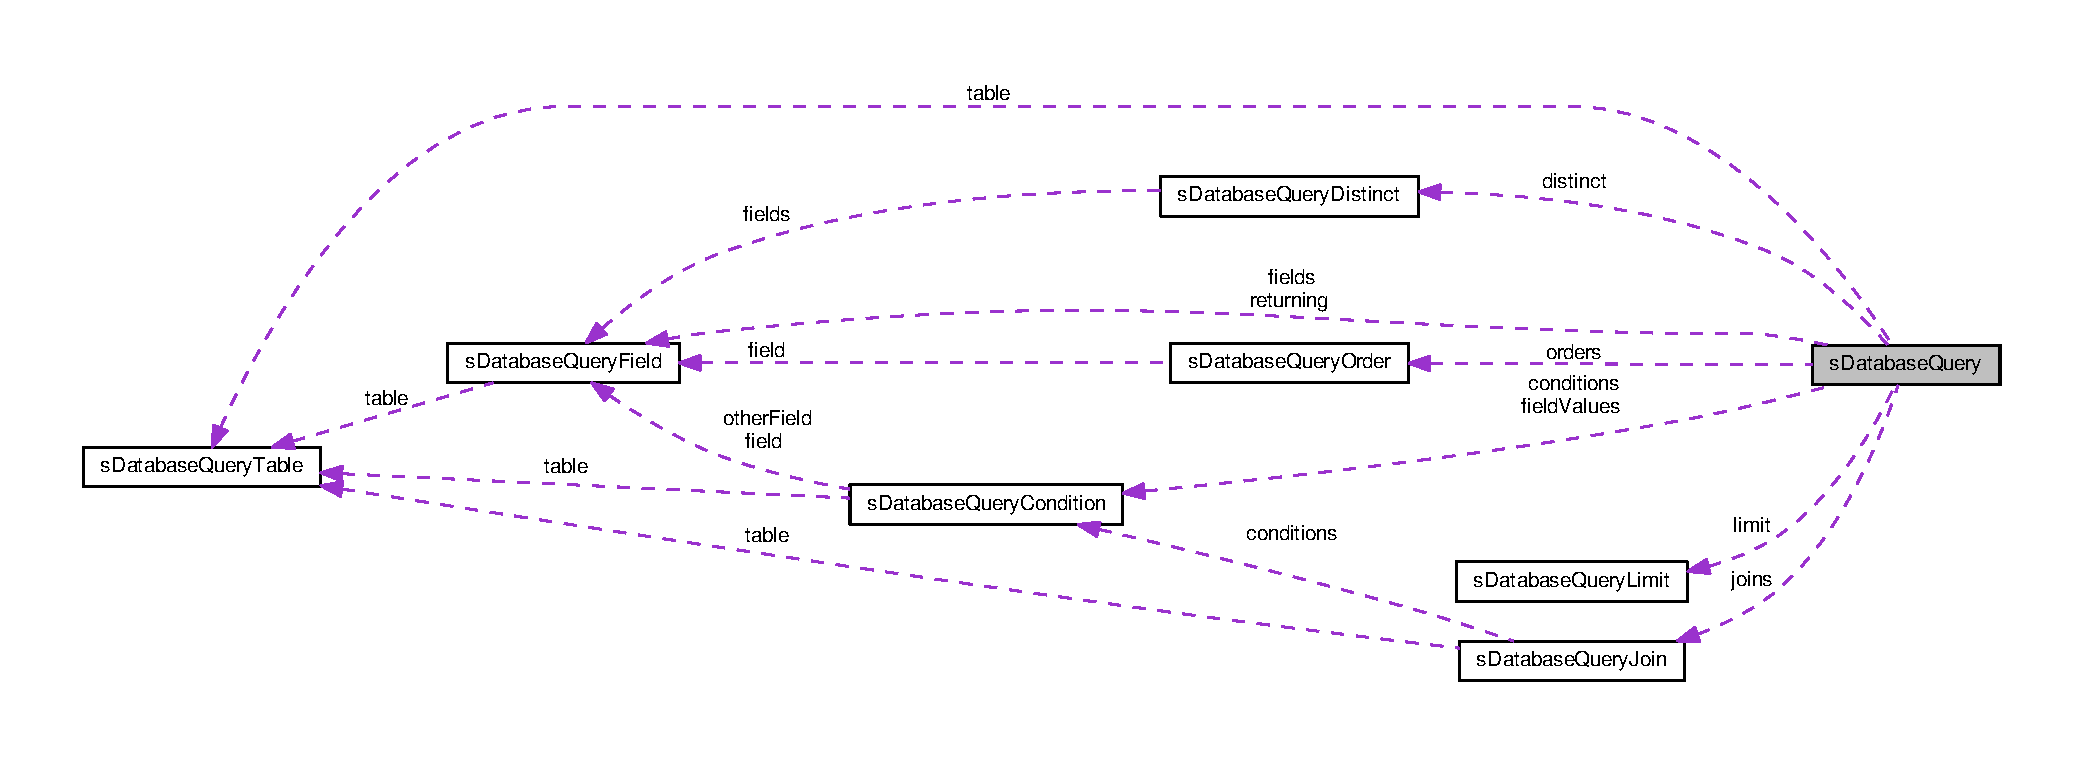
\includegraphics[width=350pt]{structsDatabaseQuery__coll__graph}
\end{center}
\end{figure}
\subsection*{Atrybuty publiczne}
\begin{DoxyCompactItemize}
\item 
\hyperlink{structsDatabaseQueryTable}{Database\+Query\+Table} $\ast$ \hyperlink{structsDatabaseQuery_a8d34ce4ad0e31c1bc8978ec03d4b5fbf}{table}
\item 
\hyperlink{structsDatabaseQueryDistinct}{Database\+Query\+Distinct} $\ast$ \hyperlink{structsDatabaseQuery_af873390ab854ce4a34f704971d271521}{distinct}
\item 
\hyperlink{structsDatabaseQueryField}{Database\+Query\+Field} $\ast$$\ast$ \hyperlink{structsDatabaseQuery_a2075e002e2ecbf166d9fbcc6f9780701}{fields}
\item 
unsigned int \hyperlink{structsDatabaseQuery_a052737bce106f2758ba5d5ac663ff57a}{fields\+Size}
\item 
\hyperlink{structsDatabaseQueryCondition}{Database\+Query\+Field\+Value} $\ast$$\ast$ \hyperlink{structsDatabaseQuery_a7bf7cf5cda36b6c6d3701926c35d8972}{field\+Values}
\item 
unsigned int \hyperlink{structsDatabaseQuery_aa203f0cb4e33b39d48e6674250d9f74d}{field\+Values\+Size}
\item 
\hyperlink{structsDatabaseQueryCondition}{Database\+Query\+Condition} $\ast$$\ast$ \hyperlink{structsDatabaseQuery_a54e52c15ffef2b87e3b2c7a4d0ffc2f9}{conditions}
\item 
unsigned int \hyperlink{structsDatabaseQuery_a7534216a1d5ad726447b73b6eb4fdbc4}{conditions\+Size}
\item 
\hyperlink{structsDatabaseQueryJoin}{Database\+Query\+Join} $\ast$$\ast$ \hyperlink{structsDatabaseQuery_aa66192f20c6390fd1bd5f2db96860926}{joins}
\item 
unsigned int \hyperlink{structsDatabaseQuery_aca409db9b76aea5d1e83390e2a251fd3}{joins\+Size}
\item 
\hyperlink{structsDatabaseQueryField}{Database\+Query\+Field} $\ast$$\ast$ \hyperlink{structsDatabaseQuery_ad88d21177dbe929109914b4b75665454}{returning}
\item 
unsigned int \hyperlink{structsDatabaseQuery_a08dafb08cb00fac230eaceb0dfd20c9f}{returning\+Size}
\item 
\hyperlink{structsDatabaseQueryOrder}{Database\+Query\+Order} $\ast$$\ast$ \hyperlink{structsDatabaseQuery_a4f2d3a55d0e7fcd151f7650c08ff7975}{orders}
\item 
unsigned int \hyperlink{structsDatabaseQuery_aecb5648962f556532a3a2c91b4970397}{orders\+Size}
\item 
\hyperlink{structsDatabaseQueryLimit}{Database\+Query\+Limit} $\ast$ \hyperlink{structsDatabaseQuery_aeca8178bae8fc02faae2bf64d6e7455a}{limit}
\item 
Database\+Query\+Type \hyperlink{structsDatabaseQuery_a5b7daf6543a0c36ab9b6a2a948f953bb}{type}
\end{DoxyCompactItemize}


\subsection{Opis szczegółowy}
Full query data 

\subsection{Dokumentacja atrybutów składowych}
\index{s\+Database\+Query@{s\+Database\+Query}!conditions@{conditions}}
\index{conditions@{conditions}!s\+Database\+Query@{s\+Database\+Query}}
\subsubsection[{\texorpdfstring{conditions}{conditions}}]{\setlength{\rightskip}{0pt plus 5cm}{\bf Database\+Query\+Condition}$\ast$$\ast$ s\+Database\+Query\+::conditions}\hypertarget{structsDatabaseQuery_a54e52c15ffef2b87e3b2c7a4d0ffc2f9}{}\label{structsDatabaseQuery_a54e52c15ffef2b87e3b2c7a4d0ffc2f9}
Conditions \index{s\+Database\+Query@{s\+Database\+Query}!conditions\+Size@{conditions\+Size}}
\index{conditions\+Size@{conditions\+Size}!s\+Database\+Query@{s\+Database\+Query}}
\subsubsection[{\texorpdfstring{conditions\+Size}{conditionsSize}}]{\setlength{\rightskip}{0pt plus 5cm}unsigned int s\+Database\+Query\+::conditions\+Size}\hypertarget{structsDatabaseQuery_a7534216a1d5ad726447b73b6eb4fdbc4}{}\label{structsDatabaseQuery_a7534216a1d5ad726447b73b6eb4fdbc4}
Number of conditions \index{s\+Database\+Query@{s\+Database\+Query}!distinct@{distinct}}
\index{distinct@{distinct}!s\+Database\+Query@{s\+Database\+Query}}
\subsubsection[{\texorpdfstring{distinct}{distinct}}]{\setlength{\rightskip}{0pt plus 5cm}{\bf Database\+Query\+Distinct}$\ast$ s\+Database\+Query\+::distinct}\hypertarget{structsDatabaseQuery_af873390ab854ce4a34f704971d271521}{}\label{structsDatabaseQuery_af873390ab854ce4a34f704971d271521}
Distinct statement \index{s\+Database\+Query@{s\+Database\+Query}!fields@{fields}}
\index{fields@{fields}!s\+Database\+Query@{s\+Database\+Query}}
\subsubsection[{\texorpdfstring{fields}{fields}}]{\setlength{\rightskip}{0pt plus 5cm}{\bf Database\+Query\+Field}$\ast$$\ast$ s\+Database\+Query\+::fields}\hypertarget{structsDatabaseQuery_a2075e002e2ecbf166d9fbcc6f9780701}{}\label{structsDatabaseQuery_a2075e002e2ecbf166d9fbcc6f9780701}
Select fields \index{s\+Database\+Query@{s\+Database\+Query}!fields\+Size@{fields\+Size}}
\index{fields\+Size@{fields\+Size}!s\+Database\+Query@{s\+Database\+Query}}
\subsubsection[{\texorpdfstring{fields\+Size}{fieldsSize}}]{\setlength{\rightskip}{0pt plus 5cm}unsigned int s\+Database\+Query\+::fields\+Size}\hypertarget{structsDatabaseQuery_a052737bce106f2758ba5d5ac663ff57a}{}\label{structsDatabaseQuery_a052737bce106f2758ba5d5ac663ff57a}
Number of fields to select \index{s\+Database\+Query@{s\+Database\+Query}!field\+Values@{field\+Values}}
\index{field\+Values@{field\+Values}!s\+Database\+Query@{s\+Database\+Query}}
\subsubsection[{\texorpdfstring{field\+Values}{fieldValues}}]{\setlength{\rightskip}{0pt plus 5cm}{\bf Database\+Query\+Field\+Value}$\ast$$\ast$ s\+Database\+Query\+::field\+Values}\hypertarget{structsDatabaseQuery_a7bf7cf5cda36b6c6d3701926c35d8972}{}\label{structsDatabaseQuery_a7bf7cf5cda36b6c6d3701926c35d8972}
Fields to update/insert \index{s\+Database\+Query@{s\+Database\+Query}!field\+Values\+Size@{field\+Values\+Size}}
\index{field\+Values\+Size@{field\+Values\+Size}!s\+Database\+Query@{s\+Database\+Query}}
\subsubsection[{\texorpdfstring{field\+Values\+Size}{fieldValuesSize}}]{\setlength{\rightskip}{0pt plus 5cm}unsigned int s\+Database\+Query\+::field\+Values\+Size}\hypertarget{structsDatabaseQuery_aa203f0cb4e33b39d48e6674250d9f74d}{}\label{structsDatabaseQuery_aa203f0cb4e33b39d48e6674250d9f74d}
Number fields to update/insert \index{s\+Database\+Query@{s\+Database\+Query}!joins@{joins}}
\index{joins@{joins}!s\+Database\+Query@{s\+Database\+Query}}
\subsubsection[{\texorpdfstring{joins}{joins}}]{\setlength{\rightskip}{0pt plus 5cm}{\bf Database\+Query\+Join}$\ast$$\ast$ s\+Database\+Query\+::joins}\hypertarget{structsDatabaseQuery_aa66192f20c6390fd1bd5f2db96860926}{}\label{structsDatabaseQuery_aa66192f20c6390fd1bd5f2db96860926}
Table to join \index{s\+Database\+Query@{s\+Database\+Query}!joins\+Size@{joins\+Size}}
\index{joins\+Size@{joins\+Size}!s\+Database\+Query@{s\+Database\+Query}}
\subsubsection[{\texorpdfstring{joins\+Size}{joinsSize}}]{\setlength{\rightskip}{0pt plus 5cm}unsigned int s\+Database\+Query\+::joins\+Size}\hypertarget{structsDatabaseQuery_aca409db9b76aea5d1e83390e2a251fd3}{}\label{structsDatabaseQuery_aca409db9b76aea5d1e83390e2a251fd3}
Number of table to join \index{s\+Database\+Query@{s\+Database\+Query}!limit@{limit}}
\index{limit@{limit}!s\+Database\+Query@{s\+Database\+Query}}
\subsubsection[{\texorpdfstring{limit}{limit}}]{\setlength{\rightskip}{0pt plus 5cm}{\bf Database\+Query\+Limit}$\ast$ s\+Database\+Query\+::limit}\hypertarget{structsDatabaseQuery_aeca8178bae8fc02faae2bf64d6e7455a}{}\label{structsDatabaseQuery_aeca8178bae8fc02faae2bf64d6e7455a}
Limit statements \index{s\+Database\+Query@{s\+Database\+Query}!orders@{orders}}
\index{orders@{orders}!s\+Database\+Query@{s\+Database\+Query}}
\subsubsection[{\texorpdfstring{orders}{orders}}]{\setlength{\rightskip}{0pt plus 5cm}{\bf Database\+Query\+Order}$\ast$$\ast$ s\+Database\+Query\+::orders}\hypertarget{structsDatabaseQuery_a4f2d3a55d0e7fcd151f7650c08ff7975}{}\label{structsDatabaseQuery_a4f2d3a55d0e7fcd151f7650c08ff7975}
Order statements \index{s\+Database\+Query@{s\+Database\+Query}!orders\+Size@{orders\+Size}}
\index{orders\+Size@{orders\+Size}!s\+Database\+Query@{s\+Database\+Query}}
\subsubsection[{\texorpdfstring{orders\+Size}{ordersSize}}]{\setlength{\rightskip}{0pt plus 5cm}unsigned int s\+Database\+Query\+::orders\+Size}\hypertarget{structsDatabaseQuery_aecb5648962f556532a3a2c91b4970397}{}\label{structsDatabaseQuery_aecb5648962f556532a3a2c91b4970397}
Number of order statements \index{s\+Database\+Query@{s\+Database\+Query}!returning@{returning}}
\index{returning@{returning}!s\+Database\+Query@{s\+Database\+Query}}
\subsubsection[{\texorpdfstring{returning}{returning}}]{\setlength{\rightskip}{0pt plus 5cm}{\bf Database\+Query\+Field}$\ast$$\ast$ s\+Database\+Query\+::returning}\hypertarget{structsDatabaseQuery_ad88d21177dbe929109914b4b75665454}{}\label{structsDatabaseQuery_ad88d21177dbe929109914b4b75665454}
Columns to return after insert \index{s\+Database\+Query@{s\+Database\+Query}!returning\+Size@{returning\+Size}}
\index{returning\+Size@{returning\+Size}!s\+Database\+Query@{s\+Database\+Query}}
\subsubsection[{\texorpdfstring{returning\+Size}{returningSize}}]{\setlength{\rightskip}{0pt plus 5cm}unsigned int s\+Database\+Query\+::returning\+Size}\hypertarget{structsDatabaseQuery_a08dafb08cb00fac230eaceb0dfd20c9f}{}\label{structsDatabaseQuery_a08dafb08cb00fac230eaceb0dfd20c9f}
Number of columns to return after insert \index{s\+Database\+Query@{s\+Database\+Query}!table@{table}}
\index{table@{table}!s\+Database\+Query@{s\+Database\+Query}}
\subsubsection[{\texorpdfstring{table}{table}}]{\setlength{\rightskip}{0pt plus 5cm}{\bf Database\+Query\+Table}$\ast$ s\+Database\+Query\+::table}\hypertarget{structsDatabaseQuery_a8d34ce4ad0e31c1bc8978ec03d4b5fbf}{}\label{structsDatabaseQuery_a8d34ce4ad0e31c1bc8978ec03d4b5fbf}
Main table \index{s\+Database\+Query@{s\+Database\+Query}!type@{type}}
\index{type@{type}!s\+Database\+Query@{s\+Database\+Query}}
\subsubsection[{\texorpdfstring{type}{type}}]{\setlength{\rightskip}{0pt plus 5cm}Database\+Query\+Type s\+Database\+Query\+::type}\hypertarget{structsDatabaseQuery_a5b7daf6543a0c36ab9b6a2a948f953bb}{}\label{structsDatabaseQuery_a5b7daf6543a0c36ab9b6a2a948f953bb}
Type of query 

Dokumentacja dla tej struktury została wygenerowana z pliku\+:\begin{DoxyCompactItemize}
\item 
database\+\_\+query.\+h\end{DoxyCompactItemize}

\hypertarget{structsDatabaseQueryCondition}{}\section{Dokumentacja struktury s\+Database\+Query\+Condition}
\label{structsDatabaseQueryCondition}\index{s\+Database\+Query\+Condition@{s\+Database\+Query\+Condition}}


{\ttfamily \#include $<$database\+\_\+query.\+h$>$}



Diagram współpracy dla s\+Database\+Query\+Condition\+:\nopagebreak
\begin{figure}[H]
\begin{center}
\leavevmode
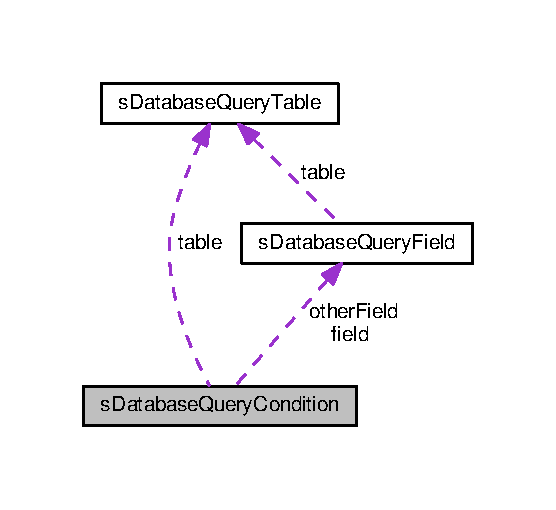
\includegraphics[width=267pt]{structsDatabaseQueryCondition__coll__graph}
\end{center}
\end{figure}
\subsection*{Atrybuty publiczne}
\begin{DoxyCompactItemize}
\item 
\hyperlink{structsDatabaseQueryTable}{Database\+Query\+Table} $\ast$ {\bfseries table}\hypertarget{structsDatabaseQueryCondition_a5b0abcb43e1a341d7fe41cd2fb234c00}{}\label{structsDatabaseQueryCondition_a5b0abcb43e1a341d7fe41cd2fb234c00}

\item 
\hyperlink{structsDatabaseQueryField}{Database\+Query\+Field} $\ast$ {\bfseries field}\hypertarget{structsDatabaseQueryCondition_a0899760067fd45e1e4a8924eed57e819}{}\label{structsDatabaseQueryCondition_a0899760067fd45e1e4a8924eed57e819}

\item 
\begin{tabbing}
xx\=xx\=xx\=xx\=xx\=xx\=xx\=xx\=xx\=\kill
union \{\\
\>char $\ast$ {\bfseries value}\\
\>char $\ast$ {\bfseries pure}\\
\>\hyperlink{structsDatabaseQueryField}{DatabaseQueryField} $\ast$ {\bfseries otherField}\\
\}; \hypertarget{structsDatabaseQueryCondition_acc2dfbe9fa14322203a54d89a9d467c5}{}\label{structsDatabaseQueryCondition_acc2dfbe9fa14322203a54d89a9d467c5}
\\

\end{tabbing}\item 
char $\ast$ {\bfseries operator}\hypertarget{structsDatabaseQueryCondition_aa252b90ac14f012ce02078dda403309d}{}\label{structsDatabaseQueryCondition_aa252b90ac14f012ce02078dda403309d}

\item 
Database\+Query\+Condition\+Type {\bfseries type}\hypertarget{structsDatabaseQueryCondition_a0d735a2c898a27fad8367293125349e6}{}\label{structsDatabaseQueryCondition_a0d735a2c898a27fad8367293125349e6}

\end{DoxyCompactItemize}


\subsection{Opis szczegółowy}
Condition data 

Dokumentacja dla tej struktury została wygenerowana z pliku\+:\begin{DoxyCompactItemize}
\item 
database\+\_\+query.\+h\end{DoxyCompactItemize}

\hypertarget{structsDatabaseQueryDistinct}{}\section{Dokumentacja struktury s\+Database\+Query\+Distinct}
\label{structsDatabaseQueryDistinct}\index{s\+Database\+Query\+Distinct@{s\+Database\+Query\+Distinct}}


{\ttfamily \#include $<$database\+\_\+query.\+h$>$}



Diagram współpracy dla s\+Database\+Query\+Distinct\+:\nopagebreak
\begin{figure}[H]
\begin{center}
\leavevmode
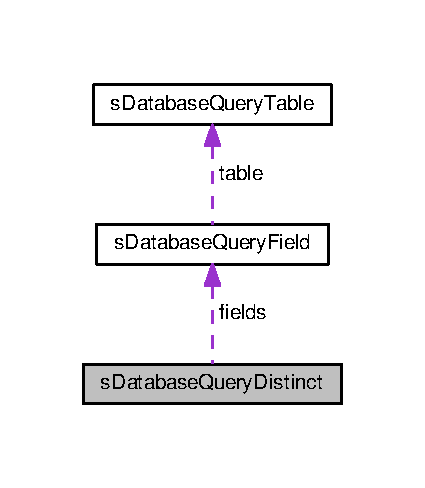
\includegraphics[width=204pt]{structsDatabaseQueryDistinct__coll__graph}
\end{center}
\end{figure}
\subsection*{Atrybuty publiczne}
\begin{DoxyCompactItemize}
\item 
\hyperlink{structsDatabaseQueryField}{Database\+Query\+Field} $\ast$$\ast$ {\bfseries fields}\hypertarget{structsDatabaseQueryDistinct_a78ff1f92d133772c3c310dec754cfa60}{}\label{structsDatabaseQueryDistinct_a78ff1f92d133772c3c310dec754cfa60}

\item 
unsigned int {\bfseries fields\+Size}\hypertarget{structsDatabaseQueryDistinct_adefbf680f57431d687f31f2f1a0ba04b}{}\label{structsDatabaseQueryDistinct_adefbf680f57431d687f31f2f1a0ba04b}

\end{DoxyCompactItemize}


\subsection{Opis szczegółowy}
Distinct on data 

Dokumentacja dla tej struktury została wygenerowana z pliku\+:\begin{DoxyCompactItemize}
\item 
database\+\_\+query.\+h\end{DoxyCompactItemize}

\hypertarget{structsDatabaseQueryField}{}\section{s\+Database\+Query\+Field Struct Reference}
\label{structsDatabaseQueryField}\index{s\+Database\+Query\+Field@{s\+Database\+Query\+Field}}


{\ttfamily \#include $<$database\+\_\+query.\+h$>$}



Collaboration diagram for s\+Database\+Query\+Field\+:\nopagebreak
\begin{figure}[H]
\begin{center}
\leavevmode
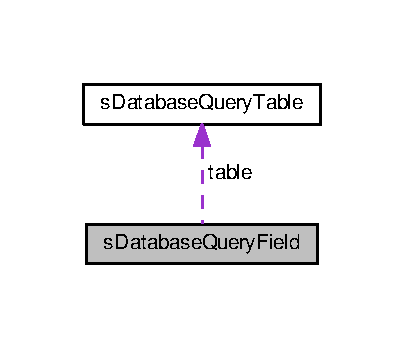
\includegraphics[width=194pt]{structsDatabaseQueryField__coll__graph}
\end{center}
\end{figure}
\subsection*{Public Attributes}
\begin{DoxyCompactItemize}
\item 
char $\ast$ \hyperlink{structsDatabaseQueryField_a89dd83131d90a8d8aeabfcafdde956b0}{name}
\item 
char $\ast$ \hyperlink{structsDatabaseQueryField_a97d3648cdd9355173c5e1f2322050473}{as}
\item 
\hyperlink{database__query_8h_a38971f81715db3c243144b5e840c2457}{Database\+Query\+Table} $\ast$ \hyperlink{structsDatabaseQueryField_a32161fc1b757bde0390ae5f3ef50c7c4}{table}
\item 
\hyperlink{json_8h_af761d54284482a1af5a01d8f52845b49}{J\+S\+O\+N\+Type} \hyperlink{structsDatabaseQueryField_a6e0fe90cd89abdc82116cc61be5119d5}{json\+Type}
\end{DoxyCompactItemize}


\subsection{Detailed Description}
Queried table column data. \begin{Desc}
\item[Examples\+: ]\par
\hyperlink{_2home_2eraden_2code_2eraden_2kore_query_2database_exec_8h-example}{/home/eraden/code/eraden/kore\+\_\+query/database\+\_\+exec.\+h}, and \hyperlink{_2home_2eraden_2code_2eraden_2kore_query_2database_query_8h-example}{/home/eraden/code/eraden/kore\+\_\+query/database\+\_\+query.\+h}.\end{Desc}


\subsection{Member Data Documentation}
\index{s\+Database\+Query\+Field@{s\+Database\+Query\+Field}!as@{as}}
\index{as@{as}!s\+Database\+Query\+Field@{s\+Database\+Query\+Field}}
\subsubsection[{\texorpdfstring{as}{as}}]{\setlength{\rightskip}{0pt plus 5cm}char$\ast$ s\+Database\+Query\+Field\+::as}\hypertarget{structsDatabaseQueryField_a97d3648cdd9355173c5e1f2322050473}{}\label{structsDatabaseQueryField_a97d3648cdd9355173c5e1f2322050473}
used by exec to fetch data \index{s\+Database\+Query\+Field@{s\+Database\+Query\+Field}!json\+Type@{json\+Type}}
\index{json\+Type@{json\+Type}!s\+Database\+Query\+Field@{s\+Database\+Query\+Field}}
\subsubsection[{\texorpdfstring{json\+Type}{jsonType}}]{\setlength{\rightskip}{0pt plus 5cm}{\bf J\+S\+O\+N\+Type} s\+Database\+Query\+Field\+::json\+Type}\hypertarget{structsDatabaseQueryField_a6e0fe90cd89abdc82116cc61be5119d5}{}\label{structsDatabaseQueryField_a6e0fe90cd89abdc82116cc61be5119d5}
how data will be fetched \index{s\+Database\+Query\+Field@{s\+Database\+Query\+Field}!name@{name}}
\index{name@{name}!s\+Database\+Query\+Field@{s\+Database\+Query\+Field}}
\subsubsection[{\texorpdfstring{name}{name}}]{\setlength{\rightskip}{0pt plus 5cm}char$\ast$ s\+Database\+Query\+Field\+::name}\hypertarget{structsDatabaseQueryField_a89dd83131d90a8d8aeabfcafdde956b0}{}\label{structsDatabaseQueryField_a89dd83131d90a8d8aeabfcafdde956b0}
column name \index{s\+Database\+Query\+Field@{s\+Database\+Query\+Field}!table@{table}}
\index{table@{table}!s\+Database\+Query\+Field@{s\+Database\+Query\+Field}}
\subsubsection[{\texorpdfstring{table}{table}}]{\setlength{\rightskip}{0pt plus 5cm}{\bf Database\+Query\+Table}$\ast$ s\+Database\+Query\+Field\+::table}\hypertarget{structsDatabaseQueryField_a32161fc1b757bde0390ae5f3ef50c7c4}{}\label{structsDatabaseQueryField_a32161fc1b757bde0390ae5f3ef50c7c4}
column table name 

The documentation for this struct was generated from the following file\+:\begin{DoxyCompactItemize}
\item 
\hyperlink{database__query_8h}{database\+\_\+query.\+h}\end{DoxyCompactItemize}

\hypertarget{structsDatabaseQueryJoin}{}\section{s\+Database\+Query\+Join Struct Reference}
\label{structsDatabaseQueryJoin}\index{s\+Database\+Query\+Join@{s\+Database\+Query\+Join}}


{\ttfamily \#include $<$database\+\_\+query.\+h$>$}



Collaboration diagram for s\+Database\+Query\+Join\+:\nopagebreak
\begin{figure}[H]
\begin{center}
\leavevmode
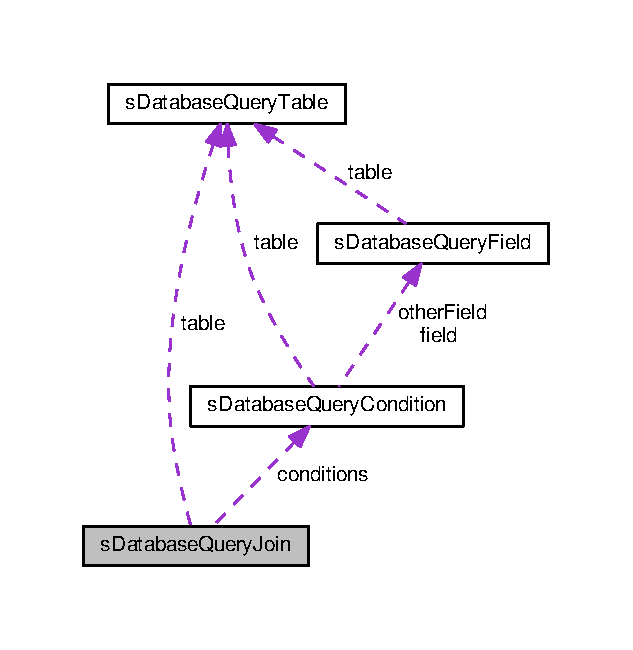
\includegraphics[width=304pt]{structsDatabaseQueryJoin__coll__graph}
\end{center}
\end{figure}
\subsection*{Public Attributes}
\begin{DoxyCompactItemize}
\item 
\hyperlink{database__query_8h_a38971f81715db3c243144b5e840c2457}{Database\+Query\+Table} $\ast$ \hyperlink{structsDatabaseQueryJoin_acbf5a41cfc09cd83a76141f6c9062917}{table}
\item 
\hyperlink{database__query_8h_a6266221c78d9f12aa27ae522162f414f}{Database\+Query\+Condition} $\ast$$\ast$ \hyperlink{structsDatabaseQueryJoin_a0c9a74a0b86f72c5b70caae49d39fd05}{conditions}
\item 
unsigned int \hyperlink{structsDatabaseQueryJoin_a5e0ea926de3b76b97479d26be2f5d935}{conditions\+Size}
\item 
\hyperlink{database__query_8h_abd7f182a993afec8e1b9946d52eafbbd}{Database\+Query\+Join\+Type} \hyperlink{structsDatabaseQueryJoin_ad0a33e6334f09c044be0d360d87cf21e}{type}
\end{DoxyCompactItemize}


\subsection{Detailed Description}
Join data \begin{Desc}
\item[Examples\+: ]\par
\hyperlink{_2home_2eraden_2code_2eraden_2kore_query_2database_query_8h-example}{/home/eraden/code/eraden/kore\+\_\+query/database\+\_\+query.\+h}.\end{Desc}


\subsection{Member Data Documentation}
\index{s\+Database\+Query\+Join@{s\+Database\+Query\+Join}!conditions@{conditions}}
\index{conditions@{conditions}!s\+Database\+Query\+Join@{s\+Database\+Query\+Join}}
\subsubsection[{\texorpdfstring{conditions}{conditions}}]{\setlength{\rightskip}{0pt plus 5cm}{\bf Database\+Query\+Condition}$\ast$$\ast$ s\+Database\+Query\+Join\+::conditions}\hypertarget{structsDatabaseQueryJoin_a0c9a74a0b86f72c5b70caae49d39fd05}{}\label{structsDatabaseQueryJoin_a0c9a74a0b86f72c5b70caae49d39fd05}
join {\ttfamily on} conditions \index{s\+Database\+Query\+Join@{s\+Database\+Query\+Join}!conditions\+Size@{conditions\+Size}}
\index{conditions\+Size@{conditions\+Size}!s\+Database\+Query\+Join@{s\+Database\+Query\+Join}}
\subsubsection[{\texorpdfstring{conditions\+Size}{conditionsSize}}]{\setlength{\rightskip}{0pt plus 5cm}unsigned int s\+Database\+Query\+Join\+::conditions\+Size}\hypertarget{structsDatabaseQueryJoin_a5e0ea926de3b76b97479d26be2f5d935}{}\label{structsDatabaseQueryJoin_a5e0ea926de3b76b97479d26be2f5d935}
number of join {\ttfamily on} conditions \index{s\+Database\+Query\+Join@{s\+Database\+Query\+Join}!table@{table}}
\index{table@{table}!s\+Database\+Query\+Join@{s\+Database\+Query\+Join}}
\subsubsection[{\texorpdfstring{table}{table}}]{\setlength{\rightskip}{0pt plus 5cm}{\bf Database\+Query\+Table}$\ast$ s\+Database\+Query\+Join\+::table}\hypertarget{structsDatabaseQueryJoin_acbf5a41cfc09cd83a76141f6c9062917}{}\label{structsDatabaseQueryJoin_acbf5a41cfc09cd83a76141f6c9062917}
join table \index{s\+Database\+Query\+Join@{s\+Database\+Query\+Join}!type@{type}}
\index{type@{type}!s\+Database\+Query\+Join@{s\+Database\+Query\+Join}}
\subsubsection[{\texorpdfstring{type}{type}}]{\setlength{\rightskip}{0pt plus 5cm}{\bf Database\+Query\+Join\+Type} s\+Database\+Query\+Join\+::type}\hypertarget{structsDatabaseQueryJoin_ad0a33e6334f09c044be0d360d87cf21e}{}\label{structsDatabaseQueryJoin_ad0a33e6334f09c044be0d360d87cf21e}
join type 

The documentation for this struct was generated from the following file\+:\begin{DoxyCompactItemize}
\item 
\hyperlink{database__query_8h}{database\+\_\+query.\+h}\end{DoxyCompactItemize}

\hypertarget{structsDatabaseQueryLimit}{}\section{Dokumentacja struktury s\+Database\+Query\+Limit}
\label{structsDatabaseQueryLimit}\index{s\+Database\+Query\+Limit@{s\+Database\+Query\+Limit}}


{\ttfamily \#include $<$database\+\_\+query.\+h$>$}

\subsection*{Atrybuty publiczne}
\begin{DoxyCompactItemize}
\item 
char $\ast$ {\bfseries limit}\hypertarget{structsDatabaseQueryLimit_a5b4d5190d79ffb220342d502d7a3a480}{}\label{structsDatabaseQueryLimit_a5b4d5190d79ffb220342d502d7a3a480}

\end{DoxyCompactItemize}


\subsection{Opis szczegółowy}
Query rows limit 

Dokumentacja dla tej struktury została wygenerowana z pliku\+:\begin{DoxyCompactItemize}
\item 
database\+\_\+query.\+h\end{DoxyCompactItemize}

\hypertarget{structsDatabaseQueryOrder}{}\section{Dokumentacja struktury s\+Database\+Query\+Order}
\label{structsDatabaseQueryOrder}\index{s\+Database\+Query\+Order@{s\+Database\+Query\+Order}}


{\ttfamily \#include $<$database\+\_\+query.\+h$>$}



Diagram współpracy dla s\+Database\+Query\+Order\+:\nopagebreak
\begin{figure}[H]
\begin{center}
\leavevmode
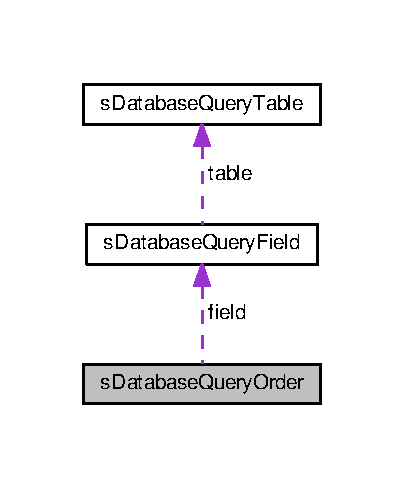
\includegraphics[width=194pt]{structsDatabaseQueryOrder__coll__graph}
\end{center}
\end{figure}
\subsection*{Atrybuty publiczne}
\begin{DoxyCompactItemize}
\item 
\hyperlink{structsDatabaseQueryField}{Database\+Query\+Field} $\ast$ {\bfseries field}\hypertarget{structsDatabaseQueryOrder_a4cfafb9043648c011721411cabb1fc22}{}\label{structsDatabaseQueryOrder_a4cfafb9043648c011721411cabb1fc22}

\item 
Database\+Query\+Order\+Direction {\bfseries direction}\hypertarget{structsDatabaseQueryOrder_a78ffc2b3348fa8f50949885229de3cad}{}\label{structsDatabaseQueryOrder_a78ffc2b3348fa8f50949885229de3cad}

\item 
char $\ast$ {\bfseries pure}\hypertarget{structsDatabaseQueryOrder_ac2b2660647eddc285042a724d03b2476}{}\label{structsDatabaseQueryOrder_ac2b2660647eddc285042a724d03b2476}

\end{DoxyCompactItemize}


\subsection{Opis szczegółowy}
Order data 

Dokumentacja dla tej struktury została wygenerowana z pliku\+:\begin{DoxyCompactItemize}
\item 
database\+\_\+query.\+h\end{DoxyCompactItemize}

\hypertarget{structsDatabaseQueryTable}{}\section{s\+Database\+Query\+Table Struct Reference}
\label{structsDatabaseQueryTable}\index{s\+Database\+Query\+Table@{s\+Database\+Query\+Table}}


{\ttfamily \#include $<$database\+\_\+query.\+h$>$}

\subsection*{Public Attributes}
\begin{DoxyCompactItemize}
\item 
char $\ast$ \hyperlink{structsDatabaseQueryTable_a4a57512c1cc994cf4cc526e55e246146}{name}
\end{DoxyCompactItemize}


\subsection{Detailed Description}
Queried table data \begin{Desc}
\item[Examples\+: ]\par
\hyperlink{_2home_2eraden_2code_2eraden_2kore_query_2database_query_8h-example}{/home/eraden/code/eraden/kore\+\_\+query/database\+\_\+query.\+h}.\end{Desc}


\subsection{Member Data Documentation}
\index{s\+Database\+Query\+Table@{s\+Database\+Query\+Table}!name@{name}}
\index{name@{name}!s\+Database\+Query\+Table@{s\+Database\+Query\+Table}}
\subsubsection[{\texorpdfstring{name}{name}}]{\setlength{\rightskip}{0pt plus 5cm}char$\ast$ s\+Database\+Query\+Table\+::name}\hypertarget{structsDatabaseQueryTable_a4a57512c1cc994cf4cc526e55e246146}{}\label{structsDatabaseQueryTable_a4a57512c1cc994cf4cc526e55e246146}
table name \begin{Desc}
\item[Examples\+: ]\par
\hyperlink{_2home_2eraden_2code_2eraden_2kore_query_2database_query_8h-example}{/home/eraden/code/eraden/kore\+\_\+query/database\+\_\+query.\+h}.\end{Desc}


The documentation for this struct was generated from the following file\+:\begin{DoxyCompactItemize}
\item 
\hyperlink{database__query_8h}{database\+\_\+query.\+h}\end{DoxyCompactItemize}

\hypertarget{structsJSON}{}\section{Dokumentacja struktury s\+J\+S\+ON}
\label{structsJSON}\index{s\+J\+S\+ON@{s\+J\+S\+ON}}


{\ttfamily \#include $<$json.\+h$>$}



Diagram współpracy dla s\+J\+S\+ON\+:\nopagebreak
\begin{figure}[H]
\begin{center}
\leavevmode
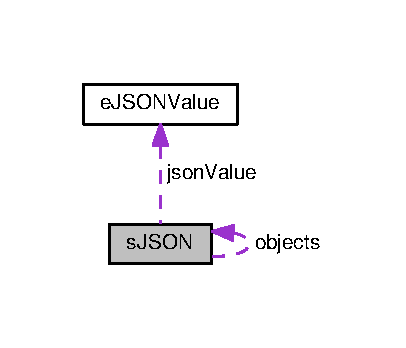
\includegraphics[width=195pt]{structsJSON__coll__graph}
\end{center}
\end{figure}
\subsection*{Atrybuty publiczne}
\begin{DoxyCompactItemize}
\item 
\hyperlink{json_8h_af761d54284482a1af5a01d8f52845b49}{J\+S\+O\+N\+Type} {\bfseries type}\hypertarget{structsJSON_addb339436be83da160932a530dce47d1}{}\label{structsJSON_addb339436be83da160932a530dce47d1}

\item 
\hyperlink{json_8h_acb7eaa79e9cdd0740c01726c3ba06e3e}{J\+S\+O\+N\+Value} \hyperlink{structsJSON_ae4d7953fe5e0369930ba3ddd91d64743}{json\+Value}
\item 
\begin{tabbing}
xx\=xx\=xx\=xx\=xx\=xx\=xx\=xx\=xx\=\kill
struct \{\\
\>\hyperlink{json_8h_a883822215fcdb974b95ff5339b5ecab4}{JSON} $\ast$$\ast$ {\bfseries objects}\\
\>char $\ast$$\ast$ \hyperlink{structsJSON_a3db035c9589ee45acad7efa117cbf1a7}{keys}\\
\>unsigned int \hyperlink{structsJSON_a0180ac53bd69e91ecfa80ace5a1c3f91}{len}\\
\} \hyperlink{structsJSON_a3c49fa17c184d6be197b183d759c4585}{children}\\

\end{tabbing}\item 
\begin{tabbing}
xx\=xx\=xx\=xx\=xx\=xx\=xx\=xx\=xx\=\kill
struct \{\\
\>\hyperlink{json_8h_a883822215fcdb974b95ff5339b5ecab4}{JSON} $\ast$$\ast$ {\bfseries objects}\\
\>unsigned int \hyperlink{structsJSON_a0180ac53bd69e91ecfa80ace5a1c3f91}{len}\\
\} \hyperlink{structsJSON_a4c8ba3fc09489bdb99aca27ef7fff535}{array}\\

\end{tabbing}\end{DoxyCompactItemize}


\subsection{Opis szczegółowy}
J\+S\+ON data \begin{Desc}
\item[Przykłady\+: ]\par
\hyperlink{_2home_2eraden_2code_2eraden_2kore_query_2json_8h-example}{/home/eraden/code/eraden/kore\+\_\+query/json.\+h}.\end{Desc}


\subsection{Dokumentacja atrybutów składowych}
\index{s\+J\+S\+ON@{s\+J\+S\+ON}!array@{array}}
\index{array@{array}!s\+J\+S\+ON@{s\+J\+S\+ON}}
\subsubsection[{\texorpdfstring{array}{array}}]{\setlength{\rightskip}{0pt plus 5cm}struct \{ ... \}   s\+J\+S\+O\+N\+::array}\hypertarget{structsJSON_a4c8ba3fc09489bdb99aca27ef7fff535}{}\label{structsJSON_a4c8ba3fc09489bdb99aca27ef7fff535}
object children \index{s\+J\+S\+ON@{s\+J\+S\+ON}!children@{children}}
\index{children@{children}!s\+J\+S\+ON@{s\+J\+S\+ON}}
\subsubsection[{\texorpdfstring{children}{children}}]{\setlength{\rightskip}{0pt plus 5cm}struct \{ ... \}   s\+J\+S\+O\+N\+::children}\hypertarget{structsJSON_a3c49fa17c184d6be197b183d759c4585}{}\label{structsJSON_a3c49fa17c184d6be197b183d759c4585}
stored value \index{s\+J\+S\+ON@{s\+J\+S\+ON}!json\+Value@{json\+Value}}
\index{json\+Value@{json\+Value}!s\+J\+S\+ON@{s\+J\+S\+ON}}
\subsubsection[{\texorpdfstring{json\+Value}{jsonValue}}]{\setlength{\rightskip}{0pt plus 5cm}{\bf J\+S\+O\+N\+Value} s\+J\+S\+O\+N\+::json\+Value}\hypertarget{structsJSON_ae4d7953fe5e0369930ba3ddd91d64743}{}\label{structsJSON_ae4d7953fe5e0369930ba3ddd91d64743}
J\+S\+ON type \index{s\+J\+S\+ON@{s\+J\+S\+ON}!keys@{keys}}
\index{keys@{keys}!s\+J\+S\+ON@{s\+J\+S\+ON}}
\subsubsection[{\texorpdfstring{keys}{keys}}]{\setlength{\rightskip}{0pt plus 5cm}char$\ast$$\ast$ s\+J\+S\+O\+N\+::keys}\hypertarget{structsJSON_a3db035c9589ee45acad7efa117cbf1a7}{}\label{structsJSON_a3db035c9589ee45acad7efa117cbf1a7}
stored objects \index{s\+J\+S\+ON@{s\+J\+S\+ON}!len@{len}}
\index{len@{len}!s\+J\+S\+ON@{s\+J\+S\+ON}}
\subsubsection[{\texorpdfstring{len}{len}}]{\setlength{\rightskip}{0pt plus 5cm}unsigned int s\+J\+S\+O\+N\+::len}\hypertarget{structsJSON_a0180ac53bd69e91ecfa80ace5a1c3f91}{}\label{structsJSON_a0180ac53bd69e91ecfa80ace5a1c3f91}
children keys

array entities 

Dokumentacja dla tej struktury została wygenerowana z pliku\+:\begin{DoxyCompactItemize}
\item 
\hyperlink{json_8h}{json.\+h}\end{DoxyCompactItemize}

\hypertarget{structsJSONPath}{}\section{s\+J\+S\+O\+N\+Path Struct Reference}
\label{structsJSONPath}\index{s\+J\+S\+O\+N\+Path@{s\+J\+S\+O\+N\+Path}}


{\ttfamily \#include $<$json.\+h$>$}

\subsection*{Public Attributes}
\begin{DoxyCompactItemize}
\item 
\begin{tabbing}
xx\=xx\=xx\=xx\=xx\=xx\=xx\=xx\=xx\=\kill
union \{\\
\>char $\ast$ \hyperlink{structsJSONPath_a7fa6192b5aea8f8f69c3a3f668129f63}{name}\\
\>unsigned \hyperlink{structsJSONPath_a0828364e7d45bd1bcca8f21b659596aa}{index}\\
\}; \hypertarget{structsJSONPath_aeed98000cbdb9665e249e21c49a6aa7a}{}\label{structsJSONPath_aeed98000cbdb9665e249e21c49a6aa7a}
\\

\end{tabbing}\item 
\hyperlink{json_8h_af761d54284482a1af5a01d8f52845b49}{J\+S\+O\+N\+Type} \hyperlink{structsJSONPath_a6c4879fb81a51a713dc7867761e3b295}{type}
\end{DoxyCompactItemize}


\subsection{Detailed Description}
Path inside json


\begin{DoxyCode}
\hyperlink{structsJSONPath}{JSONPath} path[3] = \{
    \{ .\hyperlink{structsJSONPath_a6c4879fb81a51a713dc7867761e3b295}{type}=\hyperlink{json_8h_acab6725e93cbfcfcf4273259977127a1a02bfd03b07e5b9ecd6ee0d257dc37daf}{JSON\_STRING}, .name=\textcolor{stringliteral}{"accounts"} \}, \textcolor{comment}{// for object}
    \{ .type=\hyperlink{json_8h_acab6725e93cbfcfcf4273259977127a1a6670b3c9b7ba8ab3976a7521edcc7f97}{JSON\_NUMBER}, .index=1 \}, \textcolor{comment}{// for array}
    \{ .type=\hyperlink{json_8h_acab6725e93cbfcfcf4273259977127a1aef1b2fb1bcc9012effaae713daf7b458}{JSON\_UNDEFINED}, .name=NULL \} \textcolor{comment}{// end of path}
\};
\end{DoxyCode}


\begin{DoxySeeAlso}{See also}
\hyperlink{json_8h_a6ea42f7260d5909a1287aca8676a7f3c}{J\+S\+O\+N\+\_\+find} 
\end{DoxySeeAlso}
\begin{Desc}
\item[Examples\+: ]\par
\hyperlink{_2home_2eraden_2code_2eraden_2kore_query_2json_8h-example}{/home/eraden/code/eraden/kore\+\_\+query/json.\+h}, and \hyperlink{_2home_2eraden_2code_2eraden_2kore_query_2serialize_8h-example}{/home/eraden/code/eraden/kore\+\_\+query/serialize.\+h}.\end{Desc}


\subsection{Member Data Documentation}
\index{s\+J\+S\+O\+N\+Path@{s\+J\+S\+O\+N\+Path}!index@{index}}
\index{index@{index}!s\+J\+S\+O\+N\+Path@{s\+J\+S\+O\+N\+Path}}
\subsubsection[{\texorpdfstring{index}{index}}]{\setlength{\rightskip}{0pt plus 5cm}unsigned s\+J\+S\+O\+N\+Path\+::index}\hypertarget{structsJSONPath_a0828364e7d45bd1bcca8f21b659596aa}{}\label{structsJSONPath_a0828364e7d45bd1bcca8f21b659596aa}
array index \index{s\+J\+S\+O\+N\+Path@{s\+J\+S\+O\+N\+Path}!name@{name}}
\index{name@{name}!s\+J\+S\+O\+N\+Path@{s\+J\+S\+O\+N\+Path}}
\subsubsection[{\texorpdfstring{name}{name}}]{\setlength{\rightskip}{0pt plus 5cm}char$\ast$ s\+J\+S\+O\+N\+Path\+::name}\hypertarget{structsJSONPath_a7fa6192b5aea8f8f69c3a3f668129f63}{}\label{structsJSONPath_a7fa6192b5aea8f8f69c3a3f668129f63}
object key \index{s\+J\+S\+O\+N\+Path@{s\+J\+S\+O\+N\+Path}!type@{type}}
\index{type@{type}!s\+J\+S\+O\+N\+Path@{s\+J\+S\+O\+N\+Path}}
\subsubsection[{\texorpdfstring{type}{type}}]{\setlength{\rightskip}{0pt plus 5cm}{\bf J\+S\+O\+N\+Type} s\+J\+S\+O\+N\+Path\+::type}\hypertarget{structsJSONPath_a6c4879fb81a51a713dc7867761e3b295}{}\label{structsJSONPath_a6c4879fb81a51a713dc7867761e3b295}
Path entry type \begin{Desc}
\item[Examples\+: ]\par
\hyperlink{_2home_2eraden_2code_2eraden_2kore_query_2json_8h-example}{/home/eraden/code/eraden/kore\+\_\+query/json.\+h}, and \hyperlink{_2home_2eraden_2code_2eraden_2kore_query_2serialize_8h-example}{/home/eraden/code/eraden/kore\+\_\+query/serialize.\+h}.\end{Desc}


The documentation for this struct was generated from the following file\+:\begin{DoxyCompactItemize}
\item 
\hyperlink{json_8h}{json.\+h}\end{DoxyCompactItemize}

\chapter{Dokumentacja plików}
\hypertarget{json_8h}{}\section{Dokumentacja pliku json.\+h}
\label{json_8h}\index{json.\+h@{json.\+h}}


J\+S\+ON response type.  


{\ttfamily \#include $<$string.\+h$>$}\\*
{\ttfamily \#include $<$stdio.\+h$>$}\\*
{\ttfamily \#include $<$stdlib.\+h$>$}\\*
{\ttfamily \#include \char`\"{}strings.\+h\char`\"{}}\\*
Wykres zależności załączania dla json.\+h\+:\nopagebreak
\begin{figure}[H]
\begin{center}
\leavevmode
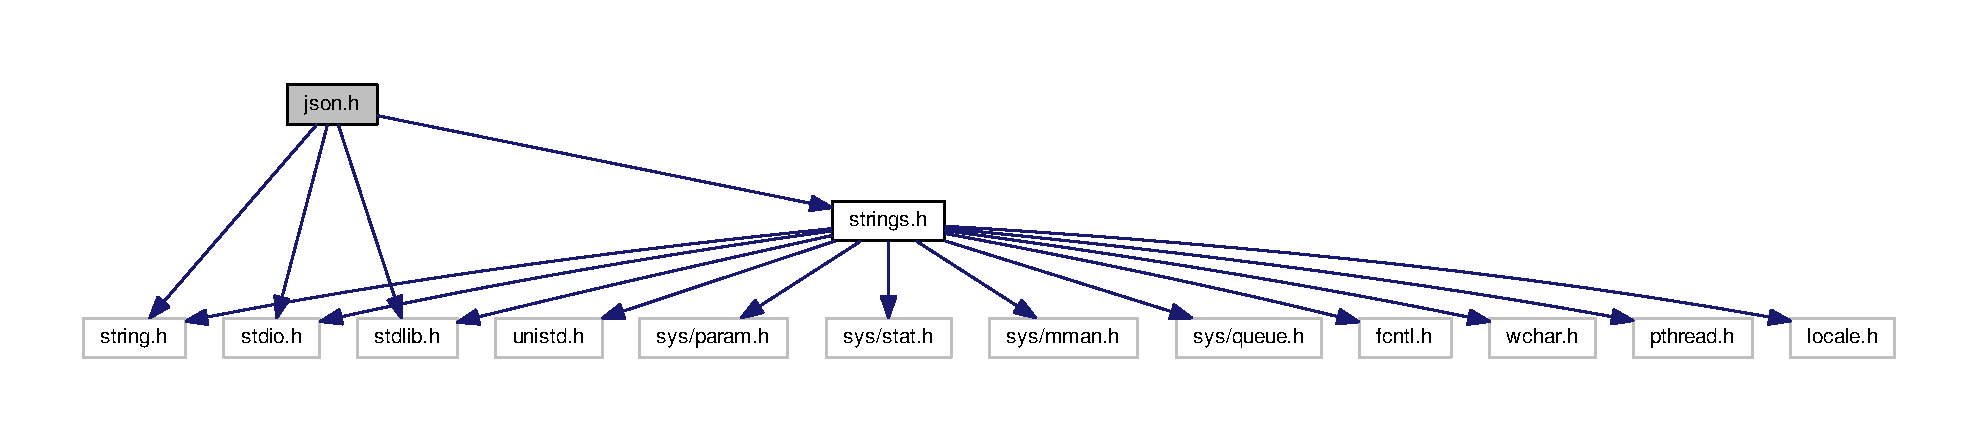
\includegraphics[width=350pt]{json_8h__incl}
\end{center}
\end{figure}
Ten wykres pokazuje, które pliki bezpośrednio lub pośrednio załączają ten plik\+:\nopagebreak
\begin{figure}[H]
\begin{center}
\leavevmode
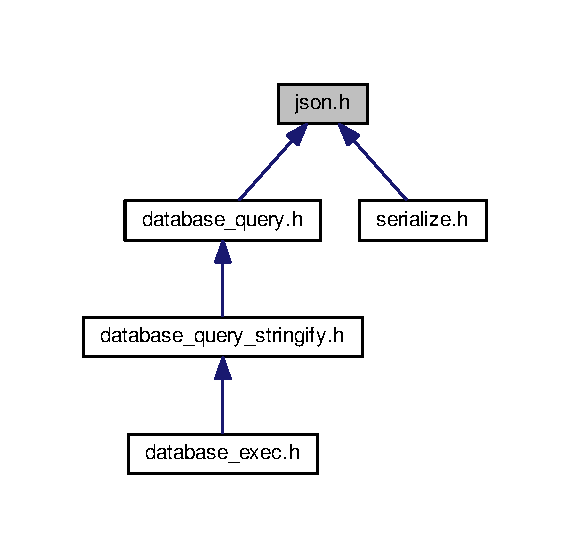
\includegraphics[width=274pt]{json_8h__dep__incl}
\end{center}
\end{figure}
\subsection*{Komponenty}
\begin{DoxyCompactItemize}
\item 
union \hyperlink{unioneJSONValue}{e\+J\+S\+O\+N\+Value}
\item 
struct \hyperlink{structsJSON}{s\+J\+S\+ON}
\item 
struct \hyperlink{structsJSONPath}{s\+J\+S\+O\+N\+Path}
\end{DoxyCompactItemize}
\subsection*{Definicje}
\begin{DoxyCompactItemize}
\item 
\#define {\bfseries J\+S\+O\+N\+\_\+\+E\+A\+C\+H\+\_\+\+P\+A\+IR}(expr,  E\+N\+T\+R\+Y\+\_\+\+K\+EY,  E\+N\+T\+R\+Y\+\_\+\+N\+A\+ME)
\item 
\#define {\bfseries J\+S\+O\+N\+\_\+\+E\+A\+C\+H\+\_\+\+P\+A\+I\+R\+\_\+\+N\+E\+XT}
\item 
\#define {\bfseries J\+S\+O\+N\+\_\+\+E\+A\+CH}(expr,  E\+N\+T\+R\+Y\+\_\+\+I\+N\+D\+EX,  E\+N\+T\+R\+Y\+\_\+\+N\+A\+ME)
\item 
\#define {\bfseries J\+S\+O\+N\+\_\+\+E\+A\+C\+H\+\_\+\+N\+E\+XT}~children\+Ptr += 1;\hypertarget{json_8h_a5b53445a30bbe35cc742b3fb4fdb16c0}{}\label{json_8h_a5b53445a30bbe35cc742b3fb4fdb16c0}

\item 
\#define {\bfseries J\+S\+O\+N\+\_\+\+E\+N\+D\+\_\+\+E\+A\+CH}~\} \} \}\hypertarget{json_8h_aaa83a532be60f2a03959b6d27bfc3625}{}\label{json_8h_aaa83a532be60f2a03959b6d27bfc3625}

\item 
\#define {\bfseries J\+S\+O\+N\+\_\+\+A\+S\+\_\+\+N\+U\+M\+B\+ER}(obj)~obj-\/$>$json\+Value.\+value\hypertarget{json_8h_af2b3f23c713d7e12cea71d2c7ce6fb04}{}\label{json_8h_af2b3f23c713d7e12cea71d2c7ce6fb04}

\item 
\#define {\bfseries J\+S\+O\+N\+\_\+\+A\+S\+\_\+\+S\+T\+R\+I\+NG}(obj)~obj-\/$>$json\+Value.\+string\hypertarget{json_8h_aaf15341d57eda1e4826b2952e9339262}{}\label{json_8h_aaf15341d57eda1e4826b2952e9339262}

\end{DoxyCompactItemize}
\subsection*{Definicje typów}
\begin{DoxyCompactItemize}
\item 
typedef struct \hyperlink{structsJSON}{s\+J\+S\+ON} \hyperlink{json_8h_a883822215fcdb974b95ff5339b5ecab4}{J\+S\+ON}
\item 
typedef struct \hyperlink{structsJSONPath}{s\+J\+S\+O\+N\+Path} \hyperlink{json_8h_a0f3747cfbfe6c68ae7b67184bd731728}{J\+S\+O\+N\+Path}
\item 
typedef enum \hyperlink{json_8h_acab6725e93cbfcfcf4273259977127a1}{e\+J\+S\+O\+N\+Type} \hyperlink{json_8h_af761d54284482a1af5a01d8f52845b49}{J\+S\+O\+N\+Type}
\item 
typedef union \hyperlink{unioneJSONValue}{e\+J\+S\+O\+N\+Value} \hyperlink{json_8h_acb7eaa79e9cdd0740c01726c3ba06e3e}{J\+S\+O\+N\+Value}
\item 
typedef enum \hyperlink{json_8h_a7a8b3184f1ecbd8fcfdb66bd9514d2b3}{e\+J\+S\+O\+N\+Clone\+Type} \hyperlink{json_8h_a82504dc7a921c3161c7fd45d4215e7b0}{J\+S\+O\+N\+Clone\+Type}
\end{DoxyCompactItemize}
\subsection*{Wyliczenia}
\begin{DoxyCompactItemize}
\item 
enum \hyperlink{json_8h_acab6725e93cbfcfcf4273259977127a1}{e\+J\+S\+O\+N\+Type} \{ \\*
{\bfseries J\+S\+O\+N\+\_\+\+U\+N\+D\+E\+F\+I\+N\+ED} = 0, 
{\bfseries J\+S\+O\+N\+\_\+\+S\+T\+R\+I\+NG} = 1, 
{\bfseries J\+S\+O\+N\+\_\+\+N\+U\+M\+B\+ER} = 1 $<$$<$ 1, 
{\bfseries J\+S\+O\+N\+\_\+\+O\+B\+J\+E\+CT} = 1 $<$$<$ 2, 
\\*
{\bfseries J\+S\+O\+N\+\_\+\+A\+R\+R\+AY} = 1 $<$$<$ 3, 
{\bfseries J\+S\+O\+N\+\_\+\+N\+U\+LL} = 1 $<$$<$ 4
 \}
\item 
enum \hyperlink{json_8h_a7a8b3184f1ecbd8fcfdb66bd9514d2b3}{e\+J\+S\+O\+N\+Clone\+Type} \{ {\bfseries J\+S\+O\+N\+\_\+\+S\+I\+M\+P\+LE} = 0, 
{\bfseries J\+S\+O\+N\+\_\+\+D\+E\+EP} = 1
 \}
\end{DoxyCompactItemize}
\subsection*{Funkcje}
\begin{DoxyCompactItemize}
\item 
\hyperlink{json_8h_a883822215fcdb974b95ff5339b5ecab4}{J\+S\+ON} $\ast$ \hyperlink{json_8h_ad8fd00eaccc81958c5a65f805e5c00ba}{J\+S\+O\+N\+\_\+alloc} (\hyperlink{json_8h_af761d54284482a1af5a01d8f52845b49}{J\+S\+O\+N\+Type} type)
\item 
\hyperlink{json_8h_a883822215fcdb974b95ff5339b5ecab4}{J\+S\+ON} $\ast$ \hyperlink{json_8h_a8564e11a595dfb8e42182c28147b1d70}{J\+S\+O\+N\+\_\+string} (char $\ast$str)
\item 
\hyperlink{json_8h_a883822215fcdb974b95ff5339b5ecab4}{J\+S\+ON} $\ast$ \hyperlink{json_8h_abcecc56303be7d8c3b1e835d058d5a2d}{J\+S\+O\+N\+\_\+number} (float n)
\item 
void \hyperlink{json_8h_ac5db034af6e012802315e2e5587a54df}{J\+S\+O\+N\+\_\+free} (\hyperlink{json_8h_a883822215fcdb974b95ff5339b5ecab4}{J\+S\+ON} $\ast$object)
\item 
\hyperlink{json_8h_a883822215fcdb974b95ff5339b5ecab4}{J\+S\+ON} $\ast$ \hyperlink{json_8h_a0b79fc03b1dffbc61cbbe9b817ef8ae6}{J\+S\+O\+N\+\_\+set} (\hyperlink{json_8h_a883822215fcdb974b95ff5339b5ecab4}{J\+S\+ON} $\ast$parent, wchar\+\_\+t $\ast$key, \hyperlink{json_8h_a883822215fcdb974b95ff5339b5ecab4}{J\+S\+ON} $\ast$json)
\item 
\hyperlink{json_8h_a883822215fcdb974b95ff5339b5ecab4}{J\+S\+ON} $\ast$ \hyperlink{json_8h_ae9460db2cd54a7462fca0aab59aaea12}{J\+S\+O\+N\+\_\+append} (\hyperlink{json_8h_a883822215fcdb974b95ff5339b5ecab4}{J\+S\+ON} $\ast$array, \hyperlink{json_8h_a883822215fcdb974b95ff5339b5ecab4}{J\+S\+ON} $\ast$entry)
\item 
char $\ast$ \hyperlink{json_8h_a88f3755b96cc3a6ca0adbd35e0092280}{J\+S\+O\+N\+\_\+stringify} (\hyperlink{json_8h_a883822215fcdb974b95ff5339b5ecab4}{J\+S\+ON} $\ast$root)
\item 
\hyperlink{json_8h_a883822215fcdb974b95ff5339b5ecab4}{J\+S\+ON} $\ast$ \hyperlink{json_8h_a6ea42f7260d5909a1287aca8676a7f3c}{J\+S\+O\+N\+\_\+find} (\hyperlink{json_8h_a883822215fcdb974b95ff5339b5ecab4}{J\+S\+ON} $\ast$source, \hyperlink{json_8h_a0f3747cfbfe6c68ae7b67184bd731728}{J\+S\+O\+N\+Path} $\ast$path)
\item 
char $\ast$ \hyperlink{json_8h_ac6e8a1f93227d3017c1e3b5e1bb03591}{J\+S\+O\+N\+\_\+escape} (char $\ast$string)
\item 
\hyperlink{json_8h_a883822215fcdb974b95ff5339b5ecab4}{J\+S\+ON} $\ast$ \hyperlink{json_8h_a5d72929696e1de3ab3b8ad39a684dded}{J\+S\+O\+N\+\_\+clone} (\hyperlink{json_8h_a883822215fcdb974b95ff5339b5ecab4}{J\+S\+ON} $\ast$obj, \hyperlink{json_8h_a82504dc7a921c3161c7fd45d4215e7b0}{J\+S\+O\+N\+Clone\+Type} deep)
\item 
int \hyperlink{json_8h_ad042d2d456ea6186716a5071c0151370}{J\+S\+O\+N\+\_\+merge\+J\+S\+ON} (\hyperlink{json_8h_a883822215fcdb974b95ff5339b5ecab4}{J\+S\+ON} $\ast$target, \hyperlink{json_8h_a883822215fcdb974b95ff5339b5ecab4}{J\+S\+ON} $\ast$source, \hyperlink{json_8h_a82504dc7a921c3161c7fd45d4215e7b0}{J\+S\+O\+N\+Clone\+Type} deep)
\item 
\hyperlink{json_8h_acb7eaa79e9cdd0740c01726c3ba06e3e}{J\+S\+O\+N\+Value} \hyperlink{json_8h_af6b5d6ad33f7765b65e275785b40ef8b}{J\+S\+O\+N\+\_\+value\+Of} (\hyperlink{json_8h_a883822215fcdb974b95ff5339b5ecab4}{J\+S\+ON} $\ast$object, char $\ast$key)
\end{DoxyCompactItemize}


\subsection{Opis szczegółowy}
J\+S\+ON response type. 

\begin{DoxyAuthor}{Autor}
Adrian Eraden Woźniak 
\end{DoxyAuthor}
\begin{DoxyDate}{Data}
21.\+12.\+2016 
\end{DoxyDate}


\subsection{Dokumentacja definicji}
\index{json.\+h@{json.\+h}!J\+S\+O\+N\+\_\+\+E\+A\+CH@{J\+S\+O\+N\+\_\+\+E\+A\+CH}}
\index{J\+S\+O\+N\+\_\+\+E\+A\+CH@{J\+S\+O\+N\+\_\+\+E\+A\+CH}!json.\+h@{json.\+h}}
\subsubsection[{\texorpdfstring{J\+S\+O\+N\+\_\+\+E\+A\+CH}{JSON_EACH}}]{\setlength{\rightskip}{0pt plus 5cm}\#define J\+S\+O\+N\+\_\+\+E\+A\+CH(
\begin{DoxyParamCaption}
\item[{}]{expr, }
\item[{}]{E\+N\+T\+R\+Y\+\_\+\+I\+N\+D\+EX, }
\item[{}]{E\+N\+T\+R\+Y\+\_\+\+N\+A\+ME}
\end{DoxyParamCaption}
)}\hypertarget{json_8h_a8e13c5cdd8813b3cfc264836b70c94f5}{}\label{json_8h_a8e13c5cdd8813b3cfc264836b70c94f5}
{\bfseries Wartość\+:}
\begin{DoxyCode}
\{ \hyperlink{json_8h_a883822215fcdb974b95ff5339b5ecab4}{\(\backslash\)}
\hyperlink{json_8h_a883822215fcdb974b95ff5339b5ecab4}{  JSON} *array = expr; \(\backslash\)
  if (array) \{ \hyperlink{json_8h_a883822215fcdb974b95ff5339b5ecab4}{\(\backslash\)}
\hyperlink{json_8h_a883822215fcdb974b95ff5339b5ecab4}{    JSON} **childrenPtr = array->\hyperlink{structsJSON_a4c8ba3fc09489bdb99aca27ef7fff535}{array}.objects; \(\backslash\)
    for (\textcolor{keywordtype}{unsigned} \textcolor{keywordtype}{int} ENTRY\_INDEX = 0; ENTRY\_INDEX < array->array.len; ENTRY\_INDEX ++) \{ 
      \hyperlink{json_8h_a883822215fcdb974b95ff5339b5ecab4}{\(\backslash\)}
\hyperlink{json_8h_a883822215fcdb974b95ff5339b5ecab4}{      JSON} *ENTRY\_NAME = *childrenPtr;
\end{DoxyCode}
\index{json.\+h@{json.\+h}!J\+S\+O\+N\+\_\+\+E\+A\+C\+H\+\_\+\+P\+A\+IR@{J\+S\+O\+N\+\_\+\+E\+A\+C\+H\+\_\+\+P\+A\+IR}}
\index{J\+S\+O\+N\+\_\+\+E\+A\+C\+H\+\_\+\+P\+A\+IR@{J\+S\+O\+N\+\_\+\+E\+A\+C\+H\+\_\+\+P\+A\+IR}!json.\+h@{json.\+h}}
\subsubsection[{\texorpdfstring{J\+S\+O\+N\+\_\+\+E\+A\+C\+H\+\_\+\+P\+A\+IR}{JSON_EACH_PAIR}}]{\setlength{\rightskip}{0pt plus 5cm}\#define J\+S\+O\+N\+\_\+\+E\+A\+C\+H\+\_\+\+P\+A\+IR(
\begin{DoxyParamCaption}
\item[{}]{expr, }
\item[{}]{E\+N\+T\+R\+Y\+\_\+\+K\+EY, }
\item[{}]{E\+N\+T\+R\+Y\+\_\+\+N\+A\+ME}
\end{DoxyParamCaption}
)}\hypertarget{json_8h_a0970d8f80a6acb5006309383a51b9ed0}{}\label{json_8h_a0970d8f80a6acb5006309383a51b9ed0}
{\bfseries Wartość\+:}
\begin{DoxyCode}
\{ \hyperlink{json_8h_a883822215fcdb974b95ff5339b5ecab4}{\(\backslash\)}
\hyperlink{json_8h_a883822215fcdb974b95ff5339b5ecab4}{  JSON} *\textcolor{keywordtype}{object} = expr; \(\backslash\)
  if (\textcolor{keywordtype}{object}) \{ \hyperlink{json_8h_a883822215fcdb974b95ff5339b5ecab4}{\(\backslash\)}
\hyperlink{json_8h_a883822215fcdb974b95ff5339b5ecab4}{    JSON} **childrenPtr = \textcolor{keywordtype}{object}->\hyperlink{structsJSON_a3c49fa17c184d6be197b183d759c4585}{children}.objects; \(\backslash\)
    char **keysPtr = \textcolor{keywordtype}{object}->\hyperlink{structsJSON_a3c49fa17c184d6be197b183d759c4585}{children}.\hyperlink{structsJSON_a3db035c9589ee45acad7efa117cbf1a7}{keys}; \(\backslash\)
    for (\textcolor{keywordtype}{unsigned} \textcolor{keywordtype}{int} childIndex = 0; childIndex < \textcolor{keywordtype}{object}->children.len; childIndex ++) \{ 
      \hyperlink{json_8h_a883822215fcdb974b95ff5339b5ecab4}{\(\backslash\)}
\hyperlink{json_8h_a883822215fcdb974b95ff5339b5ecab4}{      JSON} *ENTRY\_NAME = *childrenPtr; \(\backslash\)
      char *ENTRY\_KEY = *keysPtr; \(\backslash\)
\end{DoxyCode}
\index{json.\+h@{json.\+h}!J\+S\+O\+N\+\_\+\+E\+A\+C\+H\+\_\+\+P\+A\+I\+R\+\_\+\+N\+E\+XT@{J\+S\+O\+N\+\_\+\+E\+A\+C\+H\+\_\+\+P\+A\+I\+R\+\_\+\+N\+E\+XT}}
\index{J\+S\+O\+N\+\_\+\+E\+A\+C\+H\+\_\+\+P\+A\+I\+R\+\_\+\+N\+E\+XT@{J\+S\+O\+N\+\_\+\+E\+A\+C\+H\+\_\+\+P\+A\+I\+R\+\_\+\+N\+E\+XT}!json.\+h@{json.\+h}}
\subsubsection[{\texorpdfstring{J\+S\+O\+N\+\_\+\+E\+A\+C\+H\+\_\+\+P\+A\+I\+R\+\_\+\+N\+E\+XT}{JSON_EACH_PAIR_NEXT}}]{\setlength{\rightskip}{0pt plus 5cm}\#define J\+S\+O\+N\+\_\+\+E\+A\+C\+H\+\_\+\+P\+A\+I\+R\+\_\+\+N\+E\+XT}\hypertarget{json_8h_aac48d6b2f8f0adbbd8437de1cb273667}{}\label{json_8h_aac48d6b2f8f0adbbd8437de1cb273667}
{\bfseries Wartość\+:}
\begin{DoxyCode}
childrenPtr += 1; \(\backslash\)
      keysPtr += 1;
\end{DoxyCode}


\subsection{Dokumentacja definicji typów}
\index{json.\+h@{json.\+h}!J\+S\+ON@{J\+S\+ON}}
\index{J\+S\+ON@{J\+S\+ON}!json.\+h@{json.\+h}}
\subsubsection[{\texorpdfstring{J\+S\+ON}{JSON}}]{\setlength{\rightskip}{0pt plus 5cm}typedef struct {\bf s\+J\+S\+ON} {\bf J\+S\+ON}}\hypertarget{json_8h_a883822215fcdb974b95ff5339b5ecab4}{}\label{json_8h_a883822215fcdb974b95ff5339b5ecab4}
J\+S\+ON data \begin{Desc}
\item[Przykłady\+: ]\par
\hyperlink{_2home_2eraden_2code_2eraden_2kore_query_2json_8h-example}{/home/eraden/code/eraden/kore\+\_\+query/json.\+h}.\end{Desc}
\index{json.\+h@{json.\+h}!J\+S\+O\+N\+Clone\+Type@{J\+S\+O\+N\+Clone\+Type}}
\index{J\+S\+O\+N\+Clone\+Type@{J\+S\+O\+N\+Clone\+Type}!json.\+h@{json.\+h}}
\subsubsection[{\texorpdfstring{J\+S\+O\+N\+Clone\+Type}{JSONCloneType}}]{\setlength{\rightskip}{0pt plus 5cm}typedef enum {\bf e\+J\+S\+O\+N\+Clone\+Type}  {\bf J\+S\+O\+N\+Clone\+Type}}\hypertarget{json_8h_a82504dc7a921c3161c7fd45d4215e7b0}{}\label{json_8h_a82504dc7a921c3161c7fd45d4215e7b0}
How J\+S\+ON should be cloned Simple indicates that complex object should not clone children \begin{Desc}
\item[Przykłady\+: ]\par
\hyperlink{_2home_2eraden_2code_2eraden_2kore_query_2json_8h-example}{/home/eraden/code/eraden/kore\+\_\+query/json.\+h}.\end{Desc}
\index{json.\+h@{json.\+h}!J\+S\+O\+N\+Path@{J\+S\+O\+N\+Path}}
\index{J\+S\+O\+N\+Path@{J\+S\+O\+N\+Path}!json.\+h@{json.\+h}}
\subsubsection[{\texorpdfstring{J\+S\+O\+N\+Path}{JSONPath}}]{\setlength{\rightskip}{0pt plus 5cm}typedef struct {\bf s\+J\+S\+O\+N\+Path} {\bf J\+S\+O\+N\+Path}}\hypertarget{json_8h_a0f3747cfbfe6c68ae7b67184bd731728}{}\label{json_8h_a0f3747cfbfe6c68ae7b67184bd731728}
Path inside json


\begin{DoxyCode}
\hyperlink{structsJSONPath}{JSONPath} path[3] = \{
    \{ .type=JSON\_STRING, .name=\textcolor{stringliteral}{"accounts"} \}, \textcolor{comment}{// for object}
    \{ .type=JSON\_NUMBER, .index=1 \}, \textcolor{comment}{// for array}
    \{ .type=JSON\_UNDEFINED, .name=NULL \} \textcolor{comment}{// end of path}
\};
\end{DoxyCode}


\begin{DoxySeeAlso}{Zobacz również}
\hyperlink{json_8h_a6ea42f7260d5909a1287aca8676a7f3c}{J\+S\+O\+N\+\_\+find} 
\end{DoxySeeAlso}
\begin{Desc}
\item[Przykłady\+: ]\par
\hyperlink{_2home_2eraden_2code_2eraden_2kore_query_2json_8h-example}{/home/eraden/code/eraden/kore\+\_\+query/json.\+h}.\end{Desc}
\index{json.\+h@{json.\+h}!J\+S\+O\+N\+Type@{J\+S\+O\+N\+Type}}
\index{J\+S\+O\+N\+Type@{J\+S\+O\+N\+Type}!json.\+h@{json.\+h}}
\subsubsection[{\texorpdfstring{J\+S\+O\+N\+Type}{JSONType}}]{\setlength{\rightskip}{0pt plus 5cm}typedef enum {\bf e\+J\+S\+O\+N\+Type} {\bf J\+S\+O\+N\+Type}}\hypertarget{json_8h_af761d54284482a1af5a01d8f52845b49}{}\label{json_8h_af761d54284482a1af5a01d8f52845b49}
Type of data stored by J\+S\+ON \begin{Desc}
\item[Przykłady\+: ]\par
\hyperlink{_2home_2eraden_2code_2eraden_2kore_query_2json_8h-example}{/home/eraden/code/eraden/kore\+\_\+query/json.\+h}.\end{Desc}
\index{json.\+h@{json.\+h}!J\+S\+O\+N\+Value@{J\+S\+O\+N\+Value}}
\index{J\+S\+O\+N\+Value@{J\+S\+O\+N\+Value}!json.\+h@{json.\+h}}
\subsubsection[{\texorpdfstring{J\+S\+O\+N\+Value}{JSONValue}}]{\setlength{\rightskip}{0pt plus 5cm}typedef union {\bf e\+J\+S\+O\+N\+Value} {\bf J\+S\+O\+N\+Value}}\hypertarget{json_8h_acb7eaa79e9cdd0740c01726c3ba06e3e}{}\label{json_8h_acb7eaa79e9cdd0740c01726c3ba06e3e}
J\+S\+ON value variants \begin{Desc}
\item[Przykłady\+: ]\par
\hyperlink{_2home_2eraden_2code_2eraden_2kore_query_2json_8h-example}{/home/eraden/code/eraden/kore\+\_\+query/json.\+h}.\end{Desc}


\subsection{Dokumentacja typów wyliczanych}
\index{json.\+h@{json.\+h}!e\+J\+S\+O\+N\+Clone\+Type@{e\+J\+S\+O\+N\+Clone\+Type}}
\index{e\+J\+S\+O\+N\+Clone\+Type@{e\+J\+S\+O\+N\+Clone\+Type}!json.\+h@{json.\+h}}
\subsubsection[{\texorpdfstring{e\+J\+S\+O\+N\+Clone\+Type}{eJSONCloneType}}]{\setlength{\rightskip}{0pt plus 5cm}enum {\bf e\+J\+S\+O\+N\+Clone\+Type}}\hypertarget{json_8h_a7a8b3184f1ecbd8fcfdb66bd9514d2b3}{}\label{json_8h_a7a8b3184f1ecbd8fcfdb66bd9514d2b3}
How J\+S\+ON should be cloned Simple indicates that complex object should not clone children \index{json.\+h@{json.\+h}!e\+J\+S\+O\+N\+Type@{e\+J\+S\+O\+N\+Type}}
\index{e\+J\+S\+O\+N\+Type@{e\+J\+S\+O\+N\+Type}!json.\+h@{json.\+h}}
\subsubsection[{\texorpdfstring{e\+J\+S\+O\+N\+Type}{eJSONType}}]{\setlength{\rightskip}{0pt plus 5cm}enum {\bf e\+J\+S\+O\+N\+Type}}\hypertarget{json_8h_acab6725e93cbfcfcf4273259977127a1}{}\label{json_8h_acab6725e93cbfcfcf4273259977127a1}
Type of data stored by J\+S\+ON 

\subsection{Dokumentacja funkcji}
\index{json.\+h@{json.\+h}!J\+S\+O\+N\+\_\+alloc@{J\+S\+O\+N\+\_\+alloc}}
\index{J\+S\+O\+N\+\_\+alloc@{J\+S\+O\+N\+\_\+alloc}!json.\+h@{json.\+h}}
\subsubsection[{\texorpdfstring{J\+S\+O\+N\+\_\+alloc(\+J\+S\+O\+N\+Type type)}{JSON_alloc(JSONType type)}}]{\setlength{\rightskip}{0pt plus 5cm}{\bf J\+S\+ON}$\ast$ J\+S\+O\+N\+\_\+alloc (
\begin{DoxyParamCaption}
\item[{{\bf J\+S\+O\+N\+Type}}]{type}
\end{DoxyParamCaption}
)}\hypertarget{json_8h_ad8fd00eaccc81958c5a65f805e5c00ba}{}\label{json_8h_ad8fd00eaccc81958c5a65f805e5c00ba}
Create new empty json object with given type 
\begin{DoxyParams}{Parametry}
{\em type} & \\
\hline
\end{DoxyParams}
\begin{DoxyReturn}{Zwraca}

\end{DoxyReturn}
\begin{Desc}
\item[Przykłady\+: ]\par
\hyperlink{_2home_2eraden_2code_2eraden_2kore_query_2json_8h-example}{/home/eraden/code/eraden/kore\+\_\+query/json.\+h}.\end{Desc}
\index{json.\+h@{json.\+h}!J\+S\+O\+N\+\_\+append@{J\+S\+O\+N\+\_\+append}}
\index{J\+S\+O\+N\+\_\+append@{J\+S\+O\+N\+\_\+append}!json.\+h@{json.\+h}}
\subsubsection[{\texorpdfstring{J\+S\+O\+N\+\_\+append(\+J\+S\+O\+N $\ast$array, J\+S\+O\+N $\ast$entry)}{JSON_append(JSON *array, JSON *entry)}}]{\setlength{\rightskip}{0pt plus 5cm}{\bf J\+S\+ON}$\ast$ J\+S\+O\+N\+\_\+append (
\begin{DoxyParamCaption}
\item[{{\bf J\+S\+ON} $\ast$}]{array, }
\item[{{\bf J\+S\+ON} $\ast$}]{entry}
\end{DoxyParamCaption}
)}\hypertarget{json_8h_ae9460db2cd54a7462fca0aab59aaea12}{}\label{json_8h_ae9460db2cd54a7462fca0aab59aaea12}
Append object at end of given array


\begin{DoxyParams}{Parametry}
{\em array} & \\
\hline
{\em entry} & \\
\hline
\end{DoxyParams}
\begin{DoxyReturn}{Zwraca}

\end{DoxyReturn}

\begin{DoxyCode}
\hyperlink{structsJSON}{JSON} *user = \hyperlink{json_8h_ae9460db2cd54a7462fca0aab59aaea12}{JSON\_append}(array, \hyperlink{json_8h_ad8fd00eaccc81958c5a65f805e5c00ba}{JSON\_alloc}(JSON\_OBJECT));
\end{DoxyCode}
 \begin{Desc}
\item[Przykłady\+: ]\par
\hyperlink{_2home_2eraden_2code_2eraden_2kore_query_2json_8h-example}{/home/eraden/code/eraden/kore\+\_\+query/json.\+h}.\end{Desc}
\index{json.\+h@{json.\+h}!J\+S\+O\+N\+\_\+clone@{J\+S\+O\+N\+\_\+clone}}
\index{J\+S\+O\+N\+\_\+clone@{J\+S\+O\+N\+\_\+clone}!json.\+h@{json.\+h}}
\subsubsection[{\texorpdfstring{J\+S\+O\+N\+\_\+clone(\+J\+S\+O\+N $\ast$obj, J\+S\+O\+N\+Clone\+Type deep)}{JSON_clone(JSON *obj, JSONCloneType deep)}}]{\setlength{\rightskip}{0pt plus 5cm}{\bf J\+S\+ON}$\ast$ J\+S\+O\+N\+\_\+clone (
\begin{DoxyParamCaption}
\item[{{\bf J\+S\+ON} $\ast$}]{obj, }
\item[{{\bf J\+S\+O\+N\+Clone\+Type}}]{deep}
\end{DoxyParamCaption}
)}\hypertarget{json_8h_a5d72929696e1de3ab3b8ad39a684dded}{}\label{json_8h_a5d72929696e1de3ab3b8ad39a684dded}
New object will be created with fallowing rules\+:


\begin{DoxyParams}{Parametry}
{\em obj} & \\
\hline
{\em deep} & \\
\hline
\end{DoxyParams}
\begin{DoxyReturn}{Zwraca}
new json object
\end{DoxyReturn}

\begin{DoxyCode}
* \textcolor{keywordtype}{object} will be cloned with all keys and returned \textcolor{keywordflow}{if} deep is \textcolor{keyword}{set} to `JSON\_DEEP`, otherwise empty \textcolor{keywordtype}{object} 
      will be returned
* array will be cloned with all children and returned \textcolor{keywordflow}{if} deep is \textcolor{keyword}{set} to `JSON\_DEEP`, otherwise empty array 
      will be returned
* \textcolor{keywordtype}{string} will be cloned
* value will be preserved
\end{DoxyCode}
 \begin{Desc}
\item[Przykłady\+: ]\par
\hyperlink{_2home_2eraden_2code_2eraden_2kore_query_2json_8h-example}{/home/eraden/code/eraden/kore\+\_\+query/json.\+h}.\end{Desc}
\index{json.\+h@{json.\+h}!J\+S\+O\+N\+\_\+escape@{J\+S\+O\+N\+\_\+escape}}
\index{J\+S\+O\+N\+\_\+escape@{J\+S\+O\+N\+\_\+escape}!json.\+h@{json.\+h}}
\subsubsection[{\texorpdfstring{J\+S\+O\+N\+\_\+escape(char $\ast$string)}{JSON_escape(char *string)}}]{\setlength{\rightskip}{0pt plus 5cm}char$\ast$ J\+S\+O\+N\+\_\+escape (
\begin{DoxyParamCaption}
\item[{char $\ast$}]{string}
\end{DoxyParamCaption}
)}\hypertarget{json_8h_ac6e8a1f93227d3017c1e3b5e1bb03591}{}\label{json_8h_ac6e8a1f93227d3017c1e3b5e1bb03591}
Escape all special characters


\begin{DoxyParams}{Parametry}
{\em string} & \\
\hline
\end{DoxyParams}
\begin{DoxyReturn}{Zwraca}

\end{DoxyReturn}

\begin{DoxyCode}
\textcolor{keywordtype}{char} *escaped = \hyperlink{json_8h_ac6e8a1f93227d3017c1e3b5e1bb03591}{JSON\_escape}(\textcolor{stringliteral}{"Some paragraph\(\backslash\)n Next paragraph"});
\textcolor{comment}{// #=> "Some paragraph\(\backslash\)\(\backslash\)n Next paragraph"}
\end{DoxyCode}
 \begin{Desc}
\item[Przykłady\+: ]\par
\hyperlink{_2home_2eraden_2code_2eraden_2kore_query_2json_8h-example}{/home/eraden/code/eraden/kore\+\_\+query/json.\+h}.\end{Desc}
\index{json.\+h@{json.\+h}!J\+S\+O\+N\+\_\+find@{J\+S\+O\+N\+\_\+find}}
\index{J\+S\+O\+N\+\_\+find@{J\+S\+O\+N\+\_\+find}!json.\+h@{json.\+h}}
\subsubsection[{\texorpdfstring{J\+S\+O\+N\+\_\+find(\+J\+S\+O\+N $\ast$source, J\+S\+O\+N\+Path $\ast$path)}{JSON_find(JSON *source, JSONPath *path)}}]{\setlength{\rightskip}{0pt plus 5cm}{\bf J\+S\+ON}$\ast$ J\+S\+O\+N\+\_\+find (
\begin{DoxyParamCaption}
\item[{{\bf J\+S\+ON} $\ast$}]{source, }
\item[{{\bf J\+S\+O\+N\+Path} $\ast$}]{path}
\end{DoxyParamCaption}
)}\hypertarget{json_8h_a6ea42f7260d5909a1287aca8676a7f3c}{}\label{json_8h_a6ea42f7260d5909a1287aca8676a7f3c}
Lookup for J\+S\+ON path


\begin{DoxyParams}{Parametry}
{\em source} & \\
\hline
{\em path} & \\
\hline
\end{DoxyParams}
\begin{DoxyReturn}{Zwraca}
json object or N\+U\+LL if not found
\end{DoxyReturn}
\begin{DoxySeeAlso}{Zobacz również}
\hyperlink{json_8h_a0f3747cfbfe6c68ae7b67184bd731728}{J\+S\+O\+N\+Path}
\end{DoxySeeAlso}

\begin{DoxyCode}
\hyperlink{structsJSONPath}{JSONPath} path[4] = \{
    \{ .type=JSON\_STRING, .name=\textcolor{stringliteral}{"hello"} \},
    \{ .type=JSON\_STRING, .name=\textcolor{stringliteral}{"world"} \},
    \{ .type=JSON\_NUMBER, .index=1 \},
    \{ .type=JSON\_UNDEFINED, .name=NULL \},
\};
\hyperlink{structsJSON}{JSON} *child = \hyperlink{json_8h_a6ea42f7260d5909a1287aca8676a7f3c}{JSON\_find}(source, path);
\end{DoxyCode}
 \begin{Desc}
\item[Przykłady\+: ]\par
\hyperlink{_2home_2eraden_2code_2eraden_2kore_query_2json_8h-example}{/home/eraden/code/eraden/kore\+\_\+query/json.\+h}.\end{Desc}
\index{json.\+h@{json.\+h}!J\+S\+O\+N\+\_\+free@{J\+S\+O\+N\+\_\+free}}
\index{J\+S\+O\+N\+\_\+free@{J\+S\+O\+N\+\_\+free}!json.\+h@{json.\+h}}
\subsubsection[{\texorpdfstring{J\+S\+O\+N\+\_\+free(\+J\+S\+O\+N $\ast$object)}{JSON_free(JSON *object)}}]{\setlength{\rightskip}{0pt plus 5cm}void J\+S\+O\+N\+\_\+free (
\begin{DoxyParamCaption}
\item[{{\bf J\+S\+ON} $\ast$}]{object}
\end{DoxyParamCaption}
)}\hypertarget{json_8h_ac5db034af6e012802315e2e5587a54df}{}\label{json_8h_ac5db034af6e012802315e2e5587a54df}
Free object memory 
\begin{DoxyParams}{Parametry}
{\em object} & \\
\hline
\end{DoxyParams}
\begin{Desc}
\item[Przykłady\+: ]\par
\hyperlink{_2home_2eraden_2code_2eraden_2kore_query_2json_8h-example}{/home/eraden/code/eraden/kore\+\_\+query/json.\+h}.\end{Desc}
\index{json.\+h@{json.\+h}!J\+S\+O\+N\+\_\+merge\+J\+S\+ON@{J\+S\+O\+N\+\_\+merge\+J\+S\+ON}}
\index{J\+S\+O\+N\+\_\+merge\+J\+S\+ON@{J\+S\+O\+N\+\_\+merge\+J\+S\+ON}!json.\+h@{json.\+h}}
\subsubsection[{\texorpdfstring{J\+S\+O\+N\+\_\+merge\+J\+S\+O\+N(\+J\+S\+O\+N $\ast$target, J\+S\+O\+N $\ast$source, J\+S\+O\+N\+Clone\+Type deep)}{JSON_mergeJSON(JSON *target, JSON *source, JSONCloneType deep)}}]{\setlength{\rightskip}{0pt plus 5cm}int J\+S\+O\+N\+\_\+merge\+J\+S\+ON (
\begin{DoxyParamCaption}
\item[{{\bf J\+S\+ON} $\ast$}]{target, }
\item[{{\bf J\+S\+ON} $\ast$}]{source, }
\item[{{\bf J\+S\+O\+N\+Clone\+Type}}]{deep}
\end{DoxyParamCaption}
)}\hypertarget{json_8h_ad042d2d456ea6186716a5071c0151370}{}\label{json_8h_ad042d2d456ea6186716a5071c0151370}
Merge two object with fallowing rules\+:


\begin{DoxyParams}{Parametry}
{\em target} & \\
\hline
{\em source} & \\
\hline
{\em deep} & \\
\hline
\end{DoxyParams}
\begin{DoxyReturn}{Zwraca}
1 if succeed or 0 if not
\end{DoxyReturn}

\begin{DoxyCode}
* \textcolor{keywordtype}{object} will be cloned and merged to target \textcolor{keywordflow}{if} deep is \textcolor{keyword}{set} to `JSON\_DEEP`, otherwise empty \textcolor{keywordtype}{object} will be 
      merged
* array will be cloned and merged to target \textcolor{keywordflow}{if} deep is \textcolor{keyword}{set} to `JSON\_DEEP`, otherwise empty array will be 
      merged
* two \textcolor{keywordtype}{string} will be concatenated without any separator
* value will be replaced
\end{DoxyCode}
 \begin{Desc}
\item[Przykłady\+: ]\par
\hyperlink{_2home_2eraden_2code_2eraden_2kore_query_2json_8h-example}{/home/eraden/code/eraden/kore\+\_\+query/json.\+h}.\end{Desc}
\index{json.\+h@{json.\+h}!J\+S\+O\+N\+\_\+number@{J\+S\+O\+N\+\_\+number}}
\index{J\+S\+O\+N\+\_\+number@{J\+S\+O\+N\+\_\+number}!json.\+h@{json.\+h}}
\subsubsection[{\texorpdfstring{J\+S\+O\+N\+\_\+number(float n)}{JSON_number(float n)}}]{\setlength{\rightskip}{0pt plus 5cm}{\bf J\+S\+ON}$\ast$ J\+S\+O\+N\+\_\+number (
\begin{DoxyParamCaption}
\item[{float}]{n}
\end{DoxyParamCaption}
)}\hypertarget{json_8h_abcecc56303be7d8c3b1e835d058d5a2d}{}\label{json_8h_abcecc56303be7d8c3b1e835d058d5a2d}
Create json object from float 
\begin{DoxyParams}{Parametry}
{\em n} & \\
\hline
\end{DoxyParams}
\begin{DoxyReturn}{Zwraca}

\end{DoxyReturn}
\begin{Desc}
\item[Przykłady\+: ]\par
\hyperlink{_2home_2eraden_2code_2eraden_2kore_query_2json_8h-example}{/home/eraden/code/eraden/kore\+\_\+query/json.\+h}.\end{Desc}
\index{json.\+h@{json.\+h}!J\+S\+O\+N\+\_\+set@{J\+S\+O\+N\+\_\+set}}
\index{J\+S\+O\+N\+\_\+set@{J\+S\+O\+N\+\_\+set}!json.\+h@{json.\+h}}
\subsubsection[{\texorpdfstring{J\+S\+O\+N\+\_\+set(\+J\+S\+O\+N $\ast$parent, wchar\+\_\+t $\ast$key, J\+S\+O\+N $\ast$json)}{JSON_set(JSON *parent, wchar_t *key, JSON *json)}}]{\setlength{\rightskip}{0pt plus 5cm}{\bf J\+S\+ON}$\ast$ J\+S\+O\+N\+\_\+set (
\begin{DoxyParamCaption}
\item[{{\bf J\+S\+ON} $\ast$}]{parent, }
\item[{wchar\+\_\+t $\ast$}]{key, }
\item[{{\bf J\+S\+ON} $\ast$}]{json}
\end{DoxyParamCaption}
)}\hypertarget{json_8h_a0b79fc03b1dffbc61cbbe9b817ef8ae6}{}\label{json_8h_a0b79fc03b1dffbc61cbbe9b817ef8ae6}
Set new value for given key. Multiple values for key can exists and newest value will be at end of keys.


\begin{DoxyParams}{Parametry}
{\em parent} & \\
\hline
{\em key} & \\
\hline
{\em json} & \\
\hline
\end{DoxyParams}
\begin{DoxyReturn}{Zwraca}

\end{DoxyReturn}

\begin{DoxyCode}
\hyperlink{structsJSON}{JSON} *users = \hyperlink{json_8h_a0b79fc03b1dffbc61cbbe9b817ef8ae6}{JSON\_set}(root, L\textcolor{stringliteral}{"users"}, \hyperlink{json_8h_ad8fd00eaccc81958c5a65f805e5c00ba}{JSON\_alloc}(JSON\_ARRAY));
\end{DoxyCode}
 \begin{Desc}
\item[Przykłady\+: ]\par
\hyperlink{_2home_2eraden_2code_2eraden_2kore_query_2json_8h-example}{/home/eraden/code/eraden/kore\+\_\+query/json.\+h}.\end{Desc}
\index{json.\+h@{json.\+h}!J\+S\+O\+N\+\_\+string@{J\+S\+O\+N\+\_\+string}}
\index{J\+S\+O\+N\+\_\+string@{J\+S\+O\+N\+\_\+string}!json.\+h@{json.\+h}}
\subsubsection[{\texorpdfstring{J\+S\+O\+N\+\_\+string(char $\ast$str)}{JSON_string(char *str)}}]{\setlength{\rightskip}{0pt plus 5cm}{\bf J\+S\+ON}$\ast$ J\+S\+O\+N\+\_\+string (
\begin{DoxyParamCaption}
\item[{char $\ast$}]{str}
\end{DoxyParamCaption}
)}\hypertarget{json_8h_a8564e11a595dfb8e42182c28147b1d70}{}\label{json_8h_a8564e11a595dfb8e42182c28147b1d70}
Create json string from string 
\begin{DoxyParams}{Parametry}
{\em str} & \\
\hline
\end{DoxyParams}
\begin{DoxyReturn}{Zwraca}

\end{DoxyReturn}
\begin{Desc}
\item[Przykłady\+: ]\par
\hyperlink{_2home_2eraden_2code_2eraden_2kore_query_2json_8h-example}{/home/eraden/code/eraden/kore\+\_\+query/json.\+h}.\end{Desc}
\index{json.\+h@{json.\+h}!J\+S\+O\+N\+\_\+stringify@{J\+S\+O\+N\+\_\+stringify}}
\index{J\+S\+O\+N\+\_\+stringify@{J\+S\+O\+N\+\_\+stringify}!json.\+h@{json.\+h}}
\subsubsection[{\texorpdfstring{J\+S\+O\+N\+\_\+stringify(\+J\+S\+O\+N $\ast$root)}{JSON_stringify(JSON *root)}}]{\setlength{\rightskip}{0pt plus 5cm}char$\ast$ J\+S\+O\+N\+\_\+stringify (
\begin{DoxyParamCaption}
\item[{{\bf J\+S\+ON} $\ast$}]{root}
\end{DoxyParamCaption}
)}\hypertarget{json_8h_a88f3755b96cc3a6ca0adbd35e0092280}{}\label{json_8h_a88f3755b96cc3a6ca0adbd35e0092280}
Create string from J\+S\+ON object


\begin{DoxyParams}{Parametry}
{\em root} & \\
\hline
\end{DoxyParams}
\begin{DoxyReturn}{Zwraca}

\end{DoxyReturn}

\begin{DoxyCode}
\textcolor{keywordtype}{char} *json = \hyperlink{json_8h_a88f3755b96cc3a6ca0adbd35e0092280}{JSON\_stringify}(root);
\end{DoxyCode}
 \begin{Desc}
\item[Przykłady\+: ]\par
\hyperlink{_2home_2eraden_2code_2eraden_2kore_query_2json_8h-example}{/home/eraden/code/eraden/kore\+\_\+query/json.\+h}.\end{Desc}
\index{json.\+h@{json.\+h}!J\+S\+O\+N\+\_\+value\+Of@{J\+S\+O\+N\+\_\+value\+Of}}
\index{J\+S\+O\+N\+\_\+value\+Of@{J\+S\+O\+N\+\_\+value\+Of}!json.\+h@{json.\+h}}
\subsubsection[{\texorpdfstring{J\+S\+O\+N\+\_\+value\+Of(\+J\+S\+O\+N $\ast$object, char $\ast$key)}{JSON_valueOf(JSON *object, char *key)}}]{\setlength{\rightskip}{0pt plus 5cm}{\bf J\+S\+O\+N\+Value} J\+S\+O\+N\+\_\+value\+Of (
\begin{DoxyParamCaption}
\item[{{\bf J\+S\+ON} $\ast$}]{object, }
\item[{char $\ast$}]{key}
\end{DoxyParamCaption}
)}\hypertarget{json_8h_af6b5d6ad33f7765b65e275785b40ef8b}{}\label{json_8h_af6b5d6ad33f7765b65e275785b40ef8b}
Returns J\+S\+O\+N\+Value for given key if missing empty J\+S\+O\+N\+Value. 
\begin{DoxyParams}{Parametry}
{\em object} & \\
\hline
{\em key} & \\
\hline
\end{DoxyParams}
\begin{DoxyReturn}{Zwraca}

\end{DoxyReturn}
\begin{Desc}
\item[Przykłady\+: ]\par
\hyperlink{_2home_2eraden_2code_2eraden_2kore_query_2json_8h-example}{/home/eraden/code/eraden/kore\+\_\+query/json.\+h}.\end{Desc}

\chapter{Dokumentacja przykładów}
\hypertarget{_2home_2eraden_2code_2eraden_2kore_query_2json_8h-example}{}\section{/home/eraden/code/eraden/kore\+\_\+query/json.\+h}

\begin{DoxyCode}
\hyperlink{structsJSON}{JSON} *root = \hyperlink{json_8h_ad8fd00eaccc81958c5a65f805e5c00ba}{JSON\_alloc}(JSON\_OBJECT);
\hyperlink{structsJSON}{JSON} *array = \hyperlink{json_8h_ad8fd00eaccc81958c5a65f805e5c00ba}{JSON\_alloc}(JSON\_ARRAY);
\hyperlink{json_8h_a0b79fc03b1dffbc61cbbe9b817ef8ae6}{JSON\_set}(root, L\textcolor{stringliteral}{"users"}, array);

\textcolor{keywordflow}{for} (\textcolor{keywordtype}{int} i = 0; i < 2; i++) \{
  \hyperlink{structsJSON}{JSON} *child = \hyperlink{json_8h_ad8fd00eaccc81958c5a65f805e5c00ba}{JSON\_alloc}(JSON\_OBJECT);
  \hyperlink{json_8h_ae9460db2cd54a7462fca0aab59aaea12}{JSON\_append}(array, child);
\}

JSON\_EACH\_PAIR(root, rootKey, rootChild)
    if (strcmp(rootKey, "some-key") == 0) ...;
    JSON\_EACH\_PAIR\_NEXT
JSON\_END\_EACH

JSON\_EACH(array, arrayIndex, arrayEntry)
    if (arrayIndex != 0) kore\_log(LOG\_INFO, ", ");
    JSON\_EACH\_NEXT
JSON\_END\_EACH

\hyperlink{structsJSONPath}{JSONPath} path[3] = \{
    \{ .type=JSON\_STRING, .name=\textcolor{stringliteral}{"users"} \},
    \{ .type=JSON\_NUMBER, .index=1 \},
    \{ .type=JSON\_UNDEFINED, .name=NULL \},
\};
\hyperlink{structsJSON}{JSON} *child = \hyperlink{json_8h_a6ea42f7260d5909a1287aca8676a7f3c}{JSON\_find}(source, path);

\textcolor{keywordtype}{char} *json = \hyperlink{json_8h_a88f3755b96cc3a6ca0adbd35e0092280}{JSON\_stringify}(root); \textcolor{comment}{//=> \{"users":[\{\},\{\}]\}}
\hyperlink{json_8h_ac5db034af6e012802315e2e5587a54df}{JSON\_free}(root);
free(json);
\end{DoxyCode}



\begin{DoxyCodeInclude}

\textcolor{preprocessor}{#pragma once}

\textcolor{preprocessor}{#include <string.h>}
\textcolor{preprocessor}{#include <stdio.h>}
\textcolor{preprocessor}{#include <stdlib.h>}

\textcolor{preprocessor}{#include "strings.h"}

\textcolor{keyword}{typedef} \textcolor{keyword}{struct }\hyperlink{structsJSON}{sJSON} \hyperlink{structsJSON}{JSON};
\textcolor{keyword}{typedef} \textcolor{keyword}{struct }\hyperlink{structsJSONPath}{sJSONPath} \hyperlink{structsJSONPath}{JSONPath};
\textcolor{keyword}{typedef} \textcolor{keyword}{enum} \hyperlink{json_8h_acab6725e93cbfcfcf4273259977127a1}{eJSONType} \hyperlink{json_8h_af761d54284482a1af5a01d8f52845b49}{JSONType};
\textcolor{keyword}{typedef} \textcolor{keyword}{union }\hyperlink{unioneJSONValue}{eJSONValue} \hyperlink{unioneJSONValue}{JSONValue};

\textcolor{preprocessor}{#define JSON\_EACH\_PAIR(expr, ENTRY\_KEY, ENTRY\_NAME) \{ \(\backslash\)}
\textcolor{preprocessor}{  JSON *object = expr; \(\backslash\)}
\textcolor{preprocessor}{  if (object) \{ \(\backslash\)}
\textcolor{preprocessor}{    JSON **childrenPtr = object->children.objects; \(\backslash\)}
\textcolor{preprocessor}{    char **keysPtr = object->children.keys; \(\backslash\)}
\textcolor{preprocessor}{    for (unsigned int childIndex = 0; childIndex < object->children.len; childIndex ++) \{ \(\backslash\)}
\textcolor{preprocessor}{      JSON *ENTRY\_NAME = *childrenPtr; \(\backslash\)}
\textcolor{preprocessor}{      char *ENTRY\_KEY = *keysPtr; \(\backslash\)}
\textcolor{preprocessor}{}
\textcolor{preprocessor}{#define JSON\_EACH\_PAIR\_NEXT \(\backslash\)}
\textcolor{preprocessor}{      childrenPtr += 1; \(\backslash\)}
\textcolor{preprocessor}{      keysPtr += 1;}

\textcolor{preprocessor}{#define JSON\_EACH(expr, ENTRY\_INDEX, ENTRY\_NAME) \{ \(\backslash\)}
\textcolor{preprocessor}{  JSON *array = expr; \(\backslash\)}
\textcolor{preprocessor}{  if (array) \{ \(\backslash\)}
\textcolor{preprocessor}{    JSON **childrenPtr = array->array.objects; \(\backslash\)}
\textcolor{preprocessor}{    for (unsigned int ENTRY\_INDEX = 0; ENTRY\_INDEX < array->array.len; ENTRY\_INDEX ++) \{ \(\backslash\)}
\textcolor{preprocessor}{      JSON *ENTRY\_NAME = *childrenPtr;}

\textcolor{preprocessor}{#define JSON\_EACH\_NEXT childrenPtr += 1;}

\textcolor{preprocessor}{#define JSON\_END\_EACH \} \} \}}

\textcolor{preprocessor}{#define JSON\_AS\_NUMBER(obj) obj->jsonValue.value}
\textcolor{preprocessor}{#define JSON\_AS\_STRING(obj) obj->jsonValue.string}

\textcolor{keyword}{typedef} \textcolor{keyword}{union }\hyperlink{unioneJSONValue}{eJSONValue} \{
  \textcolor{keywordtype}{char} *string;
  \textcolor{keywordtype}{float} value;
\} \hyperlink{json_8h_acb7eaa79e9cdd0740c01726c3ba06e3e}{JSONValue};

\textcolor{keyword}{typedef} \textcolor{keyword}{enum} \hyperlink{json_8h_acab6725e93cbfcfcf4273259977127a1}{eJSONType} \{
  JSON\_UNDEFINED = 0,
  JSON\_STRING = 1,
  JSON\_NUMBER = 1 << 1,
  JSON\_OBJECT = 1 << 2,
  JSON\_ARRAY = 1 << 3,
  JSON\_NULL = 1 << 4,
\} \hyperlink{json_8h_af761d54284482a1af5a01d8f52845b49}{JSONType};

\textcolor{keyword}{typedef} \textcolor{keyword}{enum} \hyperlink{json_8h_a7a8b3184f1ecbd8fcfdb66bd9514d2b3}{eJSONCloneType} \{
  JSON\_SIMPLE = 0,
  JSON\_DEEP = 1
\} \hyperlink{json_8h_a82504dc7a921c3161c7fd45d4215e7b0}{JSONCloneType};

\textcolor{keyword}{typedef} \textcolor{keyword}{struct }\hyperlink{structsJSON}{sJSON} \{
  JSONType type; 
  \hyperlink{unioneJSONValue}{JSONValue} jsonValue; 
  \textcolor{keyword}{struct }\{
    \hyperlink{structsJSON}{JSON} **objects; 
    \textcolor{keywordtype}{char} **keys; 
    \textcolor{keywordtype}{unsigned} \textcolor{keywordtype}{int} len; 
  \} children; 
  \textcolor{keyword}{struct }\{
    \hyperlink{structsJSON}{JSON} **objects; 
    \textcolor{keywordtype}{unsigned} \textcolor{keywordtype}{int} len; 
  \} array; 
\} \hyperlink{json_8h_a883822215fcdb974b95ff5339b5ecab4}{JSON};

\textcolor{keyword}{typedef} \textcolor{keyword}{struct }\hyperlink{structsJSONPath}{sJSONPath} \{
  \textcolor{keyword}{union }\{
    \textcolor{keywordtype}{char} *name;
    \textcolor{keywordtype}{unsigned} index;
  \};
  JSONType type;
\} \hyperlink{json_8h_a0f3747cfbfe6c68ae7b67184bd731728}{JSONPath};

\hyperlink{structsJSON}{JSON} *\hyperlink{json_8h_ad8fd00eaccc81958c5a65f805e5c00ba}{JSON\_alloc}(JSONType type);

\hyperlink{structsJSON}{JSON} *\hyperlink{json_8h_a8564e11a595dfb8e42182c28147b1d70}{JSON\_string}(\textcolor{keywordtype}{char} *str);

\hyperlink{structsJSON}{JSON} *\hyperlink{json_8h_abcecc56303be7d8c3b1e835d058d5a2d}{JSON\_number}(\textcolor{keywordtype}{float} n);

\textcolor{keywordtype}{void} \hyperlink{json_8h_ac5db034af6e012802315e2e5587a54df}{JSON\_free}(\hyperlink{structsJSON}{JSON} *\textcolor{keywordtype}{object});

\hyperlink{structsJSON}{JSON} *\hyperlink{json_8h_a0b79fc03b1dffbc61cbbe9b817ef8ae6}{JSON\_set}(\hyperlink{structsJSON}{JSON} *parent, \textcolor{keywordtype}{wchar\_t} *key, \hyperlink{structsJSON}{JSON} *json);

\hyperlink{structsJSON}{JSON} *\hyperlink{json_8h_ae9460db2cd54a7462fca0aab59aaea12}{JSON\_append}(\hyperlink{structsJSON}{JSON} *array, \hyperlink{structsJSON}{JSON} *entry);

\textcolor{keywordtype}{char} *\hyperlink{json_8h_a88f3755b96cc3a6ca0adbd35e0092280}{JSON\_stringify}(\hyperlink{structsJSON}{JSON} *root);

\hyperlink{structsJSON}{JSON} *\hyperlink{json_8h_a6ea42f7260d5909a1287aca8676a7f3c}{JSON\_find}(\hyperlink{structsJSON}{JSON} *source, \hyperlink{structsJSONPath}{JSONPath} *path);

\textcolor{keywordtype}{char} *\hyperlink{json_8h_ac6e8a1f93227d3017c1e3b5e1bb03591}{JSON\_escape}(\textcolor{keywordtype}{char} *\textcolor{keywordtype}{string});

\hyperlink{structsJSON}{JSON} *\hyperlink{json_8h_a5d72929696e1de3ab3b8ad39a684dded}{JSON\_clone}(\hyperlink{structsJSON}{JSON} *obj, \hyperlink{json_8h_a82504dc7a921c3161c7fd45d4215e7b0}{JSONCloneType} deep);

\textcolor{keywordtype}{int} \hyperlink{json_8h_ad042d2d456ea6186716a5071c0151370}{JSON\_mergeJSON}(\hyperlink{structsJSON}{JSON} *target, \hyperlink{structsJSON}{JSON} *source, 
      \hyperlink{json_8h_a82504dc7a921c3161c7fd45d4215e7b0}{JSONCloneType} deep);

\hyperlink{unioneJSONValue}{JSONValue} \hyperlink{json_8h_af6b5d6ad33f7765b65e275785b40ef8b}{JSON\_valueOf}(\hyperlink{structsJSON}{JSON} *\textcolor{keywordtype}{object}, \textcolor{keywordtype}{char} *key);
\end{DoxyCodeInclude}
 
%--- End generated contents ---

% Index
\backmatter
\newpage
\phantomsection
\clearemptydoublepage
\addcontentsline{toc}{chapter}{Indeks}
\printindex

\end{document}
